
%% bare_jrnl_compsoc.tex
%% V1.4a
%% 2014/09/17
%% by Michael Shell
%% See:
%% http://www.michaelshell.org/
%% for current contact information.
%%
%% This is a skeleton file demonstrating the use of IEEEtran.cls
%% (requires IEEEtran.cls version 1.8a or later) with an IEEE
%% Computer Society journal paper.
%%
%% Support sites:
%% http://www.michaelshell.org/tex/ieeetran/
%% http://www.ctan.org/tex-archive/macros/latex/contrib/IEEEtran/
%% and
%% http://www.ieee.org/

%%*************************************************************************
%% Legal Notice:
%% This code is offered as-is without any warranty either expressed or
%% implied; without even the implied warranty of MERCHANTABILITY or
%% FITNESS FOR A PARTICULAR PURPOSE!
%% User assumes all risk.
%% In no event shall IEEE or any contributor to this code be liable for
%% any damages or losses, including, but not limited to, incidental,
%% consequential, or any other damages, resulting from the use or misuse
%% of any information contained here.
%%
%% All comments are the opinions of their respective authors and are not
%% necessarily endorsed by the IEEE.
%%
%% This work is distributed under the LaTeX Project Public License (LPPL)
%% ( http://www.latex-project.org/ ) version 1.3, and may be freely used,
%% distributed and modified. A copy of the LPPL, version 1.3, is included
%% in the base LaTeX documentation of all distributions of LaTeX released
%% 2003/12/01 or later.
%% Retain all contribution notices and credits.
%% ** Modified files should be clearly indicated as such, including  **
%% ** renaming them and changing author support contact information. **
%%
%% File list of work: IEEEtran.cls, IEEEtran_HOWTO.pdf, bare_adv.tex,
%%                    bare_conf.tex, bare_jrnl.tex, bare_conf_compsoc.tex,
%%                    bare_jrnl_compsoc.tex, bare_jrnl_transmag.tex
%%*************************************************************************


% *** Authors should verify (and, if needed, correct) their LaTeX system  ***
% *** with the testflow diagnostic prior to trusting their LaTeX platform ***
% *** with production work. IEEE's font choices and paper sizes can       ***
% *** trigger bugs that do not appear when using other class files.       ***                          ***
% The testflow support page is at:
% http://www.michaelshell.org/tex/testflow/


\documentclass[10pt,journal,compsoc,twoside]{IEEEtran}
%
% If IEEEtran.cls has not been installed into the LaTeX system files,
% manually specify the path to it like:
% \documentclass[10pt,journal,compsoc]{../sty/IEEEtran}

\ifCLASSOPTIONcompsoc
  % IEEE Computer Society needs nocompress option
  % requires cite.sty v4.0 or later (November 2003)
  \usepackage[nocompress]{cite}
\else
  % normal IEEE
  \usepackage{cite}
\fi

\usepackage{enumerate}
\usepackage{latexsym}
\usepackage{amsfonts}
\usepackage{amsmath}
\usepackage{amssymb}
\usepackage{color}
\usepackage{colortbl}
\usepackage{epsfig}
\usepackage{xspace}
\usepackage{graphicx,epstopdf}

\usepackage{subfigure}
\usepackage{balance}
%\usepackage{cite}
\usepackage[english]{babel}



% Some very useful LaTeX packages include:
% (uncomment the ones you want to load)



% *** MISC UTILITY PACKAGES ***
%
%\usepackage{ifpdf}
% Heiko Oberdiek's ifpdf.sty is very useful if you need conditional
% compilation based on whether the output is pdf or dvi.
% usage:
% \ifpdf
%   % pdf code
% \else
%   % dvi code
% \fi
% The latest version of ifpdf.sty can be obtained from:
% http://www.ctan.org/tex-archive/macros/latex/contrib/oberdiek/
% Also, note that IEEEtran.cls V1.7 and later provides a builtin
% \ifCLASSINFOpdf conditional that works the same way.
% When switching from latex to pdflatex and vice-versa, the compiler may
% have to be run twice to clear warning/error messages.






% *** CITATION PACKAGES ***
%

% cite.sty was written by Donald Arseneau
% V1.6 and later of IEEEtran pre-defines the format of the cite.sty package
% \cite{} output to follow that of IEEE. Loading the cite package will
% result in citation numbers being automatically sorted and properly
% "compressed/ranged". e.g., [1], [9], [2], [7], [5], [6] without using
% cite.sty will become [1], [2], [5]--[7], [9] using cite.sty. cite.sty's
% \cite will automatically add leading space, if needed. Use cite.sty's
% noadjust option (cite.sty V3.8 and later) if you want to turn this off
% such as if a citation ever needs to be enclosed in parenthesis.
% cite.sty is already installed on most LaTeX systems. Be sure and use
% version 5.0 (2009-03-20) and later if using hyperref.sty.
% The latest version can be obtained at:
% http://www.ctan.org/tex-archive/macros/latex/contrib/cite/
% The documentation is contained in the cite.sty file itself.
%
% Note that some packages require special options to format as the Computer
% Society requires. In particular, Computer Society  papers do not use
% compressed citation ranges as is done in typical IEEE papers
% (e.g., [1]-[4]). Instead, they list every citation separately in order
% (e.g., [1], [2], [3], [4]). To get the latter we need to load the cite
% package with the nocompress option which is supported by cite.sty v4.0
% and later. Note also the use of a CLASSOPTION conditional provided by
% IEEEtran.cls V1.7 and later.





% *** GRAPHICS RELATED PACKAGES ***
%
\ifCLASSINFOpdf
  % \usepackage[pdftex]{graphicx}
  % declare the path(s) where your graphic files are
  % \graphicspath{{../pdf/}{../jpeg/}}
  % and their extensions so you won't have to specify these with
  % every instance of \includegraphics
  % \DeclareGraphicsExtensions{.pdf,.jpeg,.png}
\else
  % or other class option (dvipsone, dvipdf, if not using dvips). graphicx
  % will default to the driver specified in the system graphics.cfg if no
  % driver is specified.
  % \usepackage[dvips]{graphicx}
  % declare the path(s) where your graphic files are
  % \graphicspath{{../eps/}}
  % and their extensions so you won't have to specify these with
  % every instance of \includegraphics
  % \DeclareGraphicsExtensions{.eps}
\fi
% graphicx was written by David Carlisle and Sebastian Rahtz. It is
% required if you want graphics, photos, etc. graphicx.sty is already
% installed on most LaTeX systems. The latest version and documentation
% can be obtained at:
% http://www.ctan.org/tex-archive/macros/latex/required/graphics/
% Another good source of documentation is "Using Imported Graphics in
% LaTeX2e" by Keith Reckdahl which can be found at:
% http://www.ctan.org/tex-archive/info/epslatex/
%
% latex, and pdflatex in dvi mode, support graphics in encapsulated
% postscript (.eps) format. pdflatex in pdf mode supports graphics
% in .pdf, .jpeg, .png and .mps (metapost) formats. Users should ensure
% that all non-photo figures use a vector format (.eps, .pdf, .mps) and
% not a bitmapped formats (.jpeg, .png). IEEE frowns on bitmapped formats
% which can result in "jaggedy"/blurry rendering of lines and letters as
% well as large increases in file sizes.
%
% You can find documentation about the pdfTeX application at:
% http://www.tug.org/applications/pdftex






% *** MATH PACKAGES ***
%
%\usepackage[cmex10]{amsmath}
% A popular package from the American Mathematical Society that provides
% many useful and powerful commands for dealing with mathematics. If using
% it, be sure to load this package with the cmex10 option to ensure that
% only type 1 fonts will utilized at all point sizes. Without this option,
% it is possible that some math symbols, particularly those within
% footnotes, will be rendered in bitmap form which will result in a
% document that can not be IEEE Xplore compliant!
%
% Also, note that the amsmath package sets \interdisplaylinepenalty to 10000
% thus preventing page breaks from occurring within multiline equations. Use:
%\interdisplaylinepenalty=2500
% after loading amsmath to restore such page breaks as IEEEtran.cls normally
% does. amsmath.sty is already installed on most LaTeX systems. The latest
% version and documentation can be obtained at:
% http://www.ctan.org/tex-archive/macros/latex/required/amslatex/math/





% *** SPECIALIZED LIST PACKAGES ***
%
%\usepackage{algorithmic}
% algorithmic.sty was written by Peter Williams and Rogerio Brito.
% This package provides an algorithmic environment fo describing algorithms.
% You can use the algorithmic environment in-text or within a figure
% environment to provide for a floating algorithm. Do NOT use the algorithm
% floating environment provided by algorithm.sty (by the same authors) or
% algorithm2e.sty (by Christophe Fiorio) as IEEE does not use dedicated
% algorithm float types and packages that provide these will not provide
% correct IEEE style captions. The latest version and documentation of
% algorithmic.sty can be obtained at:
% http://www.ctan.org/tex-archive/macros/latex/contrib/algorithms/
% There is also a support site at:
% http://algorithms.berlios.de/index.html
% Also of interest may be the (relatively newer and more customizable)
% algorithmicx.sty package by Szasz Janos:
% http://www.ctan.org/tex-archive/macros/latex/contrib/algorithmicx/




% *** ALIGNMENT PACKAGES ***
%
%\usepackage{array}
% Frank Mittelbach's and David Carlisle's array.sty patches and improves
% the standard LaTeX2e array and tabular environments to provide better
% appearance and additional user controls. As the default LaTeX2e table
% generation code is lacking to the point of almost being broken with
% respect to the quality of the end results, all users are strongly
% advised to use an enhanced (at the very least that provided by array.sty)
% set of table tools. array.sty is already installed on most systems. The
% latest version and documentation can be obtained at:
% http://www.ctan.org/tex-archive/macros/latex/required/tools/


% IEEEtran contains the IEEEeqnarray family of commands that can be used to
% generate multiline equations as well as matrices, tables, etc., of high
% quality.




% *** SUBFIGURE PACKAGES ***
%\ifCLASSOPTIONcompsoc
%  \usepackage[caption=false,font=footnotesize,labelfont=sf,textfont=sf]{subfig}
%\else
%  \usepackage[caption=false,font=footnotesize]{subfig}
%\fi
% subfig.sty, written by Steven Douglas Cochran, is the modern replacement
% for subfigure.sty, the latter of which is no longer maintained and is
% incompatible with some LaTeX packages including fixltx2e. However,
% subfig.sty requires and automatically loads Axel Sommerfeldt's caption.sty
% which will override IEEEtran.cls' handling of captions and this will result
% in non-IEEE style figure/table captions. To prevent this problem, be sure
% and invoke subfig.sty's "caption=false" package option (available since
% subfig.sty version 1.3, 2005/06/28) as this is will preserve IEEEtran.cls
% handling of captions.
% Note that the Computer Society format requires a sans serif font rather
% than the serif font used in traditional IEEE formatting and thus the need
% to invoke different subfig.sty package options depending on whether
% compsoc mode has been enabled.
%
% The latest version and documentation of subfig.sty can be obtained at:
% http://www.ctan.org/tex-archive/macros/latex/contrib/subfig/




% *** FLOAT PACKAGES ***
%
%\usepackage{fixltx2e}
% fixltx2e, the successor to the earlier fix2col.sty, was written by
% Frank Mittelbach and David Carlisle. This package corrects a few problems
% in the LaTeX2e kernel, the most notable of which is that in current
% LaTeX2e releases, the ordering of single and double column floats is not
% guaranteed to be preserved. Thus, an unpatched LaTeX2e can allow a
% single column figure to be placed prior to an earlier double column
% figure. The latest version and documentation can be found at:
% http://www.ctan.org/tex-archive/macros/latex/base/


%\usepackage{stfloats}
% stfloats.sty was written by Sigitas Tolusis. This package gives LaTeX2e
% the ability to do double column floats at the bottom of the page as well
% as the top. (e.g., "\begin{figure*}[!b]" is not normally possible in
% LaTeX2e). It also provides a command:
%\fnbelowfloat
% to enable the placement of footnotes below bottom floats (the standard
% LaTeX2e kernel puts them above bottom floats). This is an invasive package
% which rewrites many portions of the LaTeX2e float routines. It may not work
% with other packages that modify the LaTeX2e float routines. The latest
% version and documentation can be obtained at:
% http://www.ctan.org/tex-archive/macros/latex/contrib/sttools/
% Do not use the stfloats baselinefloat ability as IEEE does not allow
% \baselineskip to stretch. Authors submitting work to the IEEE should note
% that IEEE rarely uses double column equations and that authors should try
% to avoid such use. Do not be tempted to use the cuted.sty or midfloat.sty
% packages (also by Sigitas Tolusis) as IEEE does not format its papers in
% such ways.
% Do not attempt to use stfloats with fixltx2e as they are incompatible.
% Instead, use Morten Hogholm'a dblfloatfix which combines the features
% of both fixltx2e and stfloats:
%
% \usepackage{dblfloatfix}
% The latest version can be found at:
% http://www.ctan.org/tex-archive/macros/latex/contrib/dblfloatfix/




%\ifCLASSOPTIONcaptionsoff
%  \usepackage[nomarkers]{endfloat}
% \let\MYoriglatexcaption\caption
% \renewcommand{\caption}[2][\relax]{\MYoriglatexcaption[#2]{#2}}
%\fi
% endfloat.sty was written by James Darrell McCauley, Jeff Goldberg and
% Axel Sommerfeldt. This package may be useful when used in conjunction with
% IEEEtran.cls'  captionsoff option. Some IEEE journals/societies require that
% submissions have lists of figures/tables at the end of the paper and that
% figures/tables without any captions are placed on a page by themselves at
% the end of the document. If needed, the draftcls IEEEtran class option or
% \CLASSINPUTbaselinestretch interface can be used to increase the line
% spacing as well. Be sure and use the nomarkers option of endfloat to
% prevent endfloat from "marking" where the figures would have been placed
% in the text. The two hack lines of code above are a slight modification of
% that suggested by in the endfloat docs (section 8.4.1) to ensure that
% the full captions always appear in the list of figures/tables - even if
% the user used the short optional argument of \caption[]{}.
% IEEE papers do not typically make use of \caption[]'s optional argument,
% so this should not be an issue. A similar trick can be used to disable
% captions of packages such as subfig.sty that lack options to turn off
% the subcaptions:
% For subfig.sty:
% \let\MYorigsubfloat\subfloat
% \renewcommand{\subfloat}[2][\relax]{\MYorigsubfloat[]{#2}}
% However, the above trick will not work if both optional arguments of
% the \subfloat command are used. Furthermore, there needs to be a
% description of each subfigure *somewhere* and endfloat does not add
% subfigure captions to its list of figures. Thus, the best approach is to
% avoid the use of subfigure captions (many IEEE journals avoid them anyway)
% and instead reference/explain all the subfigures within the main caption.
% The latest version of endfloat.sty and its documentation can obtained at:
% http://www.ctan.org/tex-archive/macros/latex/contrib/endfloat/
%
% The IEEEtran \ifCLASSOPTIONcaptionsoff conditional can also be used
% later in the document, say, to conditionally put the References on a
% page by themselves.




% *** PDF, URL AND HYPERLINK PACKAGES ***
%
%\usepackage{url}
% url.sty was written by Donald Arseneau. It provides better support for
% handling and breaking URLs. url.sty is already installed on most LaTeX
% systems. The latest version and documentation can be obtained at:
% http://www.ctan.org/tex-archive/macros/latex/contrib/url/
% Basically, \url{my_url_here}.





% *** Do not adjust lengths that control margins, column widths, etc. ***
% *** Do not use packages that alter fonts (such as pslatex).         ***
% There should be no need to do such things with IEEEtran.cls V1.6 and later.
% (Unless specifically asked to do so by the journal or conference you plan
% to submit to, of course. )


% correct bad hyphenation here
\hyphenation{op-tical net-works semi-conduc-tor}

%%%%%%%%%%%%%%%%%%%%%%%%%%%%%%%%%%%%%
%% DO NOT DELETE!!
%%%%%%%%%%%%%%%%%%%%%%%%%%%%%%%%%%%%%
%\usepackage{tikz}
%\usetikzlibrary{trees}

\usepackage{epsfig}
\usepackage{multirow}
\usepackage{url}

%\newcommand{\eq}{\kw{eq}}

\newcommand{\rE}[1]{\kw{\small eHFD}_{#1}}
\newcommand{\rH}[1]{\kw{\small HFD}_{#1}}
\newcommand{\ab}{\allowbreak}

\sloppy
\newcommand{\rtable}[1]{\ensuremath{\mathsf{#1}}}
\newcommand{\ratt}[1]{\ensuremath{\mathit{#1}}}
\newcommand{\at}[1]{\protect\ensuremath{\mathsf{#1}}\xspace}
\newcommand{\myhrule}{\rule[.5pt]{\hsize}{.5pt}}
\newcommand{\oneurl}[1]{\texttt{#1}}
\newcommand{\eat}[1]{}
\newcommand{\tabstrut}{\rule{0pt}{4pt}\vspace{-0.1in}}
\newcommand{\stab}{\vspace{1.2ex}\noindent}
\newcommand{\sstab}{\vspace{.5ex}\noindent}
\newcommand{\match}{\rightleftharpoons}
\newcommand{\eg}{\emph{e.g.,}\xspace}
\newcommand{\ie}{\emph{i.e.,}\xspace}
\newcommand{\true}{\kw{true}}
\newcommand{\kop}{\kw{op}}
\newcommand{\nil}{\kw{nil}}
\newcommand{\Op}{\kw{Op}}
\newcommand{\proofs}{\noindent{\bf Proof sketch:\/ }}
\newcommand{\wrt}{\emph{w.r.t.}\xspace}


%%%%%%%%%%%%%%%%%%%%%%%%%%%%%%%%%%%%%%%%%%%%%%%%%%%%%%%%%%%%%%%%%%%%%%%%%%%%%%
% ALGORITHMS
%%%%%%%%%%%%%%%%%%%%%%%%%%%%%%%%%%%%%%%%%%%%%%%%%%%%%%%%%%%%%%%%%%%%%%%%%%%%%%%
\newcommand{\SELECT}{\mbox{{\bf select}}\ }
\newcommand{\FROM}{\mbox{{\bf from}\ }}
\newcommand{\WHERE}{\mbox{\bf where}\ }
\newcommand{\SUM}{\mbox{{\bf sum}}\ }
\newcommand{\GROUPBY}{\mbox{{\bf group by}}\ }
\newcommand{\HAVING}{\mbox{{\bf having}}\ }
\newcommand{\CASE}{\mbox{{\bf case}}\ }
\newcommand{\END}{\mbox{{\bf end}}\ }
\newcommand{\WHEN}{\mbox{{\bf when}}\ }
\newcommand{\EXISTS}{\mbox{{\bf exists}}\ }
\newcommand{\COUNT}{\mbox{\kw{count}}}
\newcommand{\INSERTINTO}{\mbox{{\bf insert into}}\ }
\newcommand{\UPDATE}{\mbox{{\bf update}}\ }
\newcommand{\SET}{\mbox{{\bf set}}\ }
\newcommand{\IN}{\mbox{{\bf in}}\ }
\newcommand{\If}{\mbox{\bf if}\ }
\newcommand{\Upon}{\mbox{\bf upon}\ }
\newcommand{\Send}{\mbox{\bf send}\ }
\newcommand{\Let}{\mbox{\bf let}\ }
\newcommand{\Call}{\mbox{\bf call}\ }
\newcommand{\Then}{\mbox{\bf then}\ }
\newcommand{\To}{\mbox{\bf to}\ }
\newcommand{\Else}{\mbox{\bf else}\ }
\newcommand{\ElseIf}{\mbox{\bf elseif}\ }
\newcommand{\While}{\mbox{\bf while}\ }
\newcommand{\Begin}{\mbox{\bf begin}\ }
\newcommand{\End}{\mbox{\bf end}\ }
\newcommand{\Do}{\mbox{\bf do}\ }
\newcommand{\Downto}{\mbox{\bf downto}\ }
\newcommand{\Repeat}{\mbox{\bf repeat}\ }
\newcommand{\Until}{\mbox{\bf until}\ }
\newcommand{\For}{\mbox{\bf for}\ }
\newcommand{\Each}{\mbox{\bf each}\ }

\newcommand{\ForEach}{\mbox{\bf for each}\ }
\newcommand{\Or}{\mbox{\bf or}\ }
\renewcommand{\And}{\mbox{\bf and}\ }
\newcommand{\Not}{\mbox{\bf not}\ }
\newcommand{\Break}{\mbox{\bf break}\ }
\newcommand{\Continue}{\mbox{\bf continue}\xspace}
\newcommand{\Return}{\mbox{\bf return}\ }
\newcommand{\Case}{\mbox{\bf case}\ }
\newcommand{\Of}{\mbox{\bf of}\ }
\newcommand{\EndCase}{\mbox{\bf end-case}\ }
\newcommand{\NIL}{\mbox{\em nil}}
\newcommand{\False}{\mbox{\em false}}
\newcommand{\True}{\mbox{\em true}}
\newcommand{\algAND}{{\sc and}\xspace}
\newcommand{\OR}{{\sc or}\xspace}
\newcommand{\NOT}{{\sc not}\xspace}
\newcommand{\kw}[1]{{\ensuremath {\mathsf{#1}}}\xspace}

\newcounter{ccc}
\newcommand{\bcc}{\setcounter{ccc}{1}\theccc.}
\newcommand{\icc}{\addtocounter{ccc}{1}\theccc.}
\newcommand{\checking}{{\mbox{\small\sf Checking}\xspace}}
\newcommand{\preProcessing}{{\mbox{\small\sf preProcessing}\xspace}}
\newcommand{\MCS} {\kw{MCS}}
\newcommand{\templateDB}{{\mbox{\small\sf templateDB}\xspace}}
\newcommand{\ChaseChecking}{{\mbox{\small\sf RandomChecking}\xspace}}
\newcommand{\chase}{{\mbox{\small\sf Chase}\xspace}}
\newcommand{\SAT}{{\mbox{\small\sf SAT}\xspace}}
\newcommand{\kSAT}{{\mbox{\small 3SAT}\xspace}}
\newcommand{\PropCFDSPC}{\kw{Prop{\small CFD\_SPC}}}
\newcommand{\PropCFDSPCU}{\kw{Prop{\small CFD\_SPCU}}}
\newcommand{\UnionEQs}{\kw{UnionEQs}}
\newcommand{\UnionCFDs}{\kw{UnionCFDs}}
\newcommand{\EQ}{\kw{EQ}}
\newcommand{\key}{\kw{key}}
\newcommand{\rep}{\kw{rep}}
\newcommand{\PEQ}{\kw{EQ2CFD}}
\newcommand{\Drop}{\kw{Drop}}
%\newcommand{\Res}{\kw{Res}}

\newcommand{\IND}{{\sc ind}\xspace}
\newcommand{\INDs}{{\sc ind}{\small s}\xspace}
\newcommand{\TGDs}{{\sc tgd}{\small s}\xspace}
\newcommand{\NP}{{\sc np}\xspace}
\newcommand{\DAGs}{{\sc dag}s\xspace}
\newcommand{\NC}{{\sc nc}\xspace}
\newcommand{\coNP}{co{\sc np}\xspace}
\newcommand{\PTIME}{{\sc ptime}\xspace}
\newcommand{\PSPACE}{{\sc pspace}\xspace}
\newcommand{\EXPTIME}{{\sc exptime}\xspace}
\newcommand{\NPSPACE}{{\sc npspace}\xspace}
\newcommand{\dom}{\protect\ensuremath{\mathsf{dom}}\xspace}
\newcommand{\atset}{\protect\ensuremath{\mathsf{attr}}\xspace}
\newcommand{\finatset}{\protect\ensuremath{\mathsf{finattr}}\xspace}
\newcommand{\pvar}{\protect\ensuremath{\mathsf{var\%}}\xspace}
\newcommand{\lLHS}{\protect\ensuremath{\mathsf{{\small LHS}}}\xspace}
\newcommand{\RBR}{\kw{RBR}}
\newcommand{\SQL}{{\sc sql}\xspace}
\newcommand{\XSLT}{{\sc xslt}\xspace}
\newcommand{\DBMS}{{\sc dbms}\xspace}
\newcommand{\ATG}{{\sc atg}\xspace}
\newcommand{\ATGs}{{\sc atg}{\small s}\xspace}
\newcommand{\EBI}{{\sc ebi}\xspace}
\newcommand{\GO}{{\sc go}\xspace}
\newcommand{\VEC}[1]{{\sc vec}(#1)}
\newcommand{\DAG}{{\sc dag}\xspace}
\newcommand{\XQ}{{\sc xq}\xspace}
\newcommand{\XQwc}{{\sc xq}$^{\scriptscriptstyle[*]}$\xspace}
\newcommand{\XQdes}{{\sc xq}$^{\scriptscriptstyle[//]}$\xspace}
\newcommand{\XQfull}{{\sc xq}$^{\scriptscriptstyle[*,//]}$\xspace}
\newcommand{\vect}[1]{$\langle$ #1 $\rangle$}
\newcommand{\sem}[1]{[\![#1]\!]}
\newcommand{\NN}[2]{#1\sem{#2}}
\newcommand{\e}[2]{{\mathit (#1,#2)}}
\newcommand{\ep}[2]{{\mathit (#1,#2)+}}
\newcommand{\brname}{\ensuremath{{\mathsf{N}}}}
\newcommand{\budrel}[1]{\ensuremath{{\brname_{#1}}}}
\newcommand{\budgen}[2]{\ensuremath{Q^\brname_\e{#1}{#2}}}
\newcommand{\budcut}[2]{\ensuremath{Q_\e{#1}{#2}}}
\newcommand{\R}{{\cal R}}
\newcommand{\G}{{\cal G}}
\newcommand{\I}{{\cal I}}
\newcommand{\V}{{\cal V}}
\newcommand{\E}{{\cal E}}
\newcommand{\eop}{\hspace*{\fill}\mbox{$\Box$}}     % End of proof
\newcounter{example}
\renewcommand{\theexample}{\arabic{example}}
\newenvironment{example}{
        \vspace{1.5ex}
        \refstepcounter{example}
        {\noindent\bf Example \theexample:}}{
        \eop\vspace{1.5ex}}
\def\copyrightspace{}
\renewcommand{\ni}{\noindent}
\newcommand{\comlore}[1]{\begin{minipage}{3in}\fbox{\fbox{\parbox[t]{3in}{{\vspace{2mm}\noindent \bf COMM(LORE):~
{ #1}\hfill  END.}}}}\end{minipage}\\}
\newcommand{\comwenfei}[1]{\begin{minipage}{3in}\fbox{\fbox{\parbox[t]{3in}{{\vspace{2mm}\noindent \bf COMM(WENFEI):~
{ #1}\hfill  END.}}}}\end{minipage}\\}
\newcommand{\comshuai}[1]{\begin{minipage}{3in}\fbox{\fbox{\parbox[t]{3in}{{\vspace{2mm}\noindent \bf COMM(SHUAI):~
{ #1}\hfill  END.}}}}\end{minipage}\\}
\newcommand{\nthesection}{\arabic{section}}
\newcounter{theorem}
\renewcommand{\thetheorem}{\arabic{theorem}}
\newcounter{prop}
\renewcommand{\theprop}{\arabic{theorem}}
\newcounter{lemma}
\renewcommand{\thelemma}{\arabic{theorem}}
\newcounter{cor}
\renewcommand{\thecor}{\arabic{theorem}}
\newenvironment{theorem}{\begin{em}
        \refstepcounter{theorem}
        {\vspace{1.5ex} \noindent\bf  Theorem  \thetheorem:}}{
        \end{em}\eop\vspace{1.5ex}} %\hspace*{\fill}\vspace*{1ex}}
\newenvironment{prop}{\begin{em}
        \refstepcounter{theorem}
        {\vspace{1.5ex}\noindent \bf Proposition \theprop:}}{
        \end{em}\eop\vspace{1.5ex}}%\hspace*{\fill}\vspace*{1ex}}
\newenvironment{lemma}{\begin{em}
        \refstepcounter{theorem}
        {\vspace{1ex}\noindent\bf Lemma \thelemma:}}{
        \end{em}\eop\vspace{1ex}} %\hspace*{\fill}\vspace*{1ex}}
\newenvironment{cor}{\begin{em}
        \refstepcounter{theorem}
        {\vspace{1.5ex}\noindent\bf Corollary \thecor:}}{
        \end{em}\eop\vspace{1.5ex}} %\hspace*{\fill}\vspace*{1ex}}
\newcounter{definition}[section]
\renewcommand{\thedefinition}{\nthesection.\arabic{definition}}
\newenvironment{definition}{
        \vspace{1.5ex}
        \refstepcounter{definition}
        {\noindent\bf Definition {\bf \thedefinition}:}}{\eop\vspace{1.5ex}
}
\newcounter{alg}[section]
\renewcommand{\thealg}{\nthesection.\arabic{alg}}
\newenvironment{alg}[1]{
        \refstepcounter{alg}
        {\vspace{1ex}\noindent\bf Algorithm \thealg:\, #1}}{
        \vspace*{1ex}}
\newcounter{arule}
\renewcommand{\thearule}{\arabic{arule}}
\newenvironment{arule}{
        \vspace{0.6ex}
        \refstepcounter{arule}
        {\noindent \em Rule \thearule:}}{
        }
\newcounter{claim}
\renewcommand{\theclaim}{\arabic{claim}}
\newenvironment{claim}{
        \vspace{0.6ex}
        \refstepcounter{claim}
        {\noindent\em Claim \theclaim:}}{%--{ Wenfei Fan}\\
        }
\newenvironment{proof}{
        \vspace{1ex}
        {\noindent\bf Proof:}}{\eop\vspace{1ex}}
\newenvironment{proofS}{
        \vspace{1ex}
        {\noindent\bf Proof:\ }}{\eop\vspace{1ex}}
\newenvironment{property}{
        \vspace{1ex}
        {\noindent\bf Property:}}{\eop\vspace{1ex}}

\newcommand{\RK}[2]{\mbox{(}#1, #2\mbox{)}}

\newenvironment{choice}{\left\{\begin{array}[c]{ll}}{\end{array}\right.}


% Symbol commands

\newcommand{\exa}[2]{{\tt\begin{tabbing}\hspace{#1}\=\+\kill #2\end{tabbing}}}
\newcommand{\ra}{\rightarrow}
\newcommand{\la}{\leftarrow}
\newenvironment{bi}{\begin{itemize}%\vspace{-0.5ex}
        \setlength{\topsep}{0.5ex}\setlength{\itemsep}{0ex}\vspace{0ex}}
        {\end{itemize}\vspace{-1ex}}
\newenvironment{be}{\begin{enumerate}%\vspace{-0.5ex}
        \setlength{\topsep}{0.5ex}\setlength{\itemsep}{0ex}\vspace{-1ex}}
        {\end{itemize}\vspace{-1ex}}
\newcommand{\ei}{\end{itemize}}
\newcommand{\ee}{\end{enumerate}}
\newcommand{\mat}[2]{{\begin{tabbing}\hspace{#1}\=\+\kill #2\end{tabbing}}}
\newcommand{\m}{\hspace{0.05in}}
\newcommand{\ls}{\hspace{0.1in}}
\newcommand{\beqn}{\vspace{-1ex}\begin{eqnarray*}}
\newcommand{\eeqn}{\vspace{-1ex}\end{eqnarray*}}

\newcommand{\INDGreedy}{{\sc IND-Greedy-Step}\xspace}
\newcommand{\FDGreedy}{{\sc FD-Greedy-Step}\xspace}
\newcommand{\INDRepairTup}{{\sc IND-Resolve-Tup}\xspace}
\newcommand{\FDRepairTup}{{\sc FD-Resolve-Tup}\xspace}
\newcommand{\InitEQ}{{\sc Init-EQ}\xspace}
\newcommand{\ResolveEQ}{{\sc Resolve-EQ}\xspace}
\newcommand{\JointFDINDRepair}{{\sc Joint-FD-IND-Repair}\xspace}
\newcommand{\FRP}{{\sc FRP}\xspace}
\newcommand{\class}{\protect\ensuremath{\mathsf{class}}\xspace}
\newcommand{\eq}{\protect\ensuremath{\mathsf{eq}}\xspace}
\newcommand{\cost}{\protect\ensuremath{\mathsf{cost}}\xspace}
\newcommand{\Sim}{\protect\ensuremath{\mathsf{sim}}\xspace}
\newcommand{\dis}{\protect\ensuremath{\mathsf{dis}}\xspace}
\newcommand{\se}{\protect\ensuremath{\mathsf{SE}}\xspace}
\newcommand{\icost}{\protect\ensuremath{\mathsf{inscost}}\xspace}
\newcommand{\mcost}{\protect\ensuremath{\mathsf{mgcost}}\xspace}
\newcommand{\rcost}{\protect\ensuremath{\mathsf{rescost}}\xspace}
\newcommand{\targ}{\protect\ensuremath{\mathsf{targ}}\xspace}
%\newcommand{\ts}{\protect\ensuremath{\mathsf{ts}}\xspace}
\newcommand{\lastcompute}{\protect\ensuremath{\mathsf{lastcompute}}\xspace}
\newcommand{\changed}{\protect\ensuremath{\mathsf{changed}}\xspace}
\newcommand{\new}{\protect\ensuremath{\mathbf{new}}\xspace}
\newcommand{\mtc}{\protect\ensuremath{\mathsf{mtc}}\xspace}
\newcommand{\priQ}{\protect\ensuremath{\mathsf{priQ}}\xspace}
\newcommand{\target}{\protect\ensuremath{\mathsf{target}}\xspace}
\newcommand{\unres}{\protect\ensuremath{\mathsf{unResolved}}\xspace}
\newcommand{\done}{\protect\ensuremath{\mathsf{done}}\xspace}
\newcommand{\pick}{{\sc PickNext}\xspace}
\newcommand{\pickfdfirst}{{\sc PickGreedyFDFirst}\xspace}
\newcommand{\pickfreefd}{{\sc PickGreedyFDFree}\xspace}
\newcommand{\pickgreedy}{{\sc PickGreedy}\xspace}
\newcommand{\pickfd}{{\sc pickNextFD}\xspace}
\newcommand{\rset}{\protect\ensuremath{\mathsf{rset}}\xspace}
\newcommand{\covset}{\protect\ensuremath{\mathsf{coverSet}}\xspace}
\newcommand{\violset}{\protect\ensuremath{\mathsf{violSet}}\xspace}
\newcommand{\attrset}{\protect\ensuremath{\mathsf{attr}}\xspace}
\newcommand{\fattrset}{\protect\ensuremath{\mathsf{finattr}}\xspace}

\newcommand{\pa}{\parallel}
\newcommand{\matchset}{\protect\ensuremath{\mathsf{matchSet}}\xspace}
\newcommand{\bestFix}{\protect\ensuremath{\mathsf{bestFix}}\xspace}
\newcommand{\bestCost}{\protect\ensuremath{\mathsf{bestCost}}\xspace}
\newcommand{\FDFirst}{\protect\ensuremath{\mathsf{FDFirst}}\xspace}
\newcommand{\Null}{\protect\ensuremath{\mathsf{null}}\xspace}
%\renewcommand{\default}[1]{\protect\ensuremath{\mathsf{def}(#1)}\xspace}
\newcommand{\best}[1]{\protect\ensuremath{\mathsf{best}(#1)}\xspace}

\newcommand{\ceq}{=_v}
\newcommand{\AND}{\displaystyle{\bigwedge_{i=1}^{n}}}
\newcommand{\U}[1]{\displaystyle{\bigcup_{#1}}}
\newcommand{\Sm}[1]{\displaystyle{\sum_{#1}}}
\newcommand{\wvec}[1]{\displaystyle{\widehat{#1}}}

\newcommand{\attr}[1]{\protect\ensuremath{\mathsf{#1}}\xspace}

\newcommand{\LA}{\{\!|}
\newcommand{\RA}{|\!\}}
% \newcommand{\tag}[1]{\LA #1\RA}
% \newcommand{\taga}[2]{\LA #1\ \ #2\RA}

\newcommand{\ip}{\Rightarrow_{M}}
\newcommand{\ipu}{\Rightarrow_{M_L}}
\newcommand{\ipp}{\rightarrow_{M}}
\newcommand{\ippu}{\rightarrow_{M_L}}
\newcommand{\inv}{\rightleftharpoons}
\newcommand{\vs}{\vspace{0.1in}}
\newcommand{\Nat}{\mbox{I$\!$N}}


\renewcommand{\L}{{\cal L}}
\newcommand{\md}{\sigma_d}
\newcommand{\inverse}{\sigma_d^{-1}}
\newcommand{\RX}{{\cal X}_R\xspace}
\newcommand{\XP}{{\cal X}\xspace}
\newcommand{\M}{{\cal M}}
\newcommand{\bU}{{\cal U}}
\newcommand{\Ir}{{\cal I}_r}
\newcommand{\B}{{\cal B}}
\renewcommand{\S}{S}
\newcommand{\C}{{\cal C}}
\newcommand{\A}{{\cal A}}
\renewcommand{\v}{\nu}
\renewcommand{\t}{\tau}
\newcommand{\T}{\Theta}
\newcommand{\embedding}{\kw{embedding}}
\newcommand{\expand}{\kw{expand}}
\newcommand{\kstar}{{\sc{star}}\xspace}
\newcommand{\kand}{{\sc{and}}\xspace}
\newcommand{\kor}{{\sc{or}}\xspace}
%\newcommand{\path}{\kw{path}}
\newcommand{\adom}{\kw{adom}}


\newcommand{\Att}{\kw{att}}
\newcommand{\reach}{\kw{reach}}
\newcommand{\partlist}{\kw{part}}
\newcommand{\assg}{\kw{local}}
\newcommand{\qual}{\kw{qual}}
\newcommand{\findpaths}{\kw{findpaths}}
\newcommand{\findpathsDAG}{\kw{findPaths{\sc DAG}}}
\newcommand{\findpathsrnd}{\kw{findPathsRand}}
\newcommand{\findpathsCycle}{\kw{findpathCycle}}
\newcommand{\ordered}{\kw{Ordered}}
\newcommand{\randomordered}{\kw{RandomOrdered}}
\newcommand{\qualityordered}{\kw{QualityOrdered}}
\newcommand{\randmaxind}{\kw{RandomMaxInd}}

%%%%%%%%%%%%%%%%%%%%
% Should be removed
% \newcommand{\sortedseq}{\qualityordered}
% \newcommand{\conflictrepair}{\randomordered}
% \newcommand{\indassign}{\randmaxind}
%%%%%%%%%%%%%%%%%%%%
\newcommand{\topdown}{\kw{topDown}}
\newcommand{\traverse}{\kw{traverse}}
\newcommand{\marked}{\kw{marked}}
\newcommand{\digraph}{{\sc dag}}
\newcommand{\digraphs}{{\sc dag}s}

\newcommand{\dt}{(\C, \v)}
\newcommand{\f}{f_{C \ra C'}}

\newcommand{\imp}{\vdash_{\cal I}}
\newcommand{\Sum}[1]{\displaystyle{\sum_{#1}}}
\newcommand{\MyAnd}[1]{\displaystyle{\bigwedge_{#1}}}

\newcommand{\CFD}{{\sc cfd}\xspace}
\newcommand{\CFDs}{{\sc cfd}{\small s}\xspace}
\newcommand{\CIND}{{\sc cind}\xspace}
\newcommand{\cind}{{\sc cind}}
\newcommand{\CINDs}{{\sc cind}{\small s}\xspace}
\newcommand{\FD}{{\sc fd}\xspace}
\newcommand{\FDs}{{\sc fd}{\small s}\xspace}

\newcommand{\CFDps}{{\small e}{\sc cfd}{\small s}\xspace}

\newcommand{\pCFD}{{\sc cfd$^{p}$}\xspace}
\newcommand{\pCFDs}{{\sc cfd$^{p}$}{\small s}\xspace}
\newcommand{\spCFDs}{{\sc cfd$^{p}$}{\scriptsize s}\xspace}
\newcommand{\sCFDs}{{\sc cfd}{\scriptsize s}\xspace}

\newcommand{\rdms}{{\sc dbms}\xspace}



\newcommand{\pCIND}{{\sc cind$^p$}\xspace}
\newcommand{\pCINDs}{{\sc cind$^p$}{\small s}\xspace}
\newcommand{\spCINDs}{{\sc cind$^p$}{\scriptsize s}\xspace}
\newcommand{\sCINDs}{{\sc cind}{\scriptsize s}\xspace}


\newcommand{\CTGDs}{{\sc ctgd}{\small s}\xspace}
\newcommand{\CGDs}{{\sc cgd}{\small s}\xspace}

\newcommand{\SCFD}{\Sigma_{\kw{cfd^p}}\xspace}
\newcommand{\SCIND}{\Sigma_{\kw{cind^p}}\xspace}


\newcommand{\td}[1]{\widehat{#1}}
\newcommand{\pcdata}{\kw{str}}
\newcommand{\sel}{\kw{sel}}
\newcommand{\ltar}{\ensuremath{L_{\kw{tar}}}}

\newcommand{\ltitle}[1]{\noindent{\large\bf #1}}
\newcommand{\stitle}[1]{\vspace{1.0ex} \noindent{\bf #1}}
\newcommand{\etitle}[1]{\vspace{1ex}\noindent{\em\underline{#1}}}

\newcommand{\setitle}[1]{\noindent{\em #1}}


\newcommand{\K}{{\cal K}}
\newcommand{\Ka}{{\cal K}_{abs}}
%
\newcommand{\LHS}{\kw{LHS}}
\newcommand{\RHS}{\kw{RHS}}


\renewcommand{\tabstrut}{\rule{0pt}{4pt}\vspace{-0.1in}}
\newcommand{\tabstruct}{\rule{0pt}{8pt}\\[-2ex]}


\newcommand{\tbrule}[1]{{\tt Rule}(#1)}
\newcommand{\frule}[1]{{\tt rule}(#1)}
\newcommand{\lU}{{\bf U} }


\newcommand{\W}{{\bf W}}
\newcommand{\card}[1]{\mid\! #1\!\mid}
\newcommand{\fth}{\hfill $\Box$}


\newcommand{\Inh}[1]{{\it Inh}({\tt #1})}
\newcommand{\Syn}[1]{{\it Syn}({\tt #1})}

\newcommand{\powerset}{{\cal P}}
\newcommand{\determine}{\longrightarrow}
\newcommand{\kleq}{\ll}
\renewcommand{\r}[1]{{\it rule}(#1)}
\newcommand{\MAXSAT}{{\sc maxgsat}\xspace}
\newcommand{\kOr}[1]{\displaystyle{\bigvee_{#1}}}
\newcommand{\kAND}[1]{\displaystyle{\bigwedge_{#1}}}

\newcommand{\batch}{\textsc{BatchDetect}\xspace}
\newcommand{\incre}{{\sc IncDetect}\xspace}

\newcommand{\dsize}{\kw{|D|}}
\newcommand{\noise}{\kw{noise\%}}
\newcommand{\psize}{\kw{|Tp|}}
\newcommand{\numVar}{\kw{Var\%}}
\newcommand{\change}{\kw{|$\Delta$D|}}
\newcommand{\kinserts}{$\kw{|\Delta D^+|}$\xspace}
\newcommand{\kdeletes}{$\kw{|\Delta D^-|}$\xspace}
\newcommand{\Doutputins}{$\kw{|\Delta V^+|}$\xspace}
\newcommand{\Doutputdel}{$\kw{|\Delta V^-|}$\xspace}
\newcommand{\var}{\kw{var}}
\newcommand{\Implic}{\textsc{Implication}\xspace}
\newcommand{\CSP}{\textsc{CSP}\xspace}


%%%%%%%%%%%%%%%%%%%%%%%%%%%%%%%%%%%%%%%%%%
%%%%% Loreto %%%%%%
%%%%%%%%%%%%%%%%%%%%%%%%%%%%%%%%%%%%%%%%%%

\renewcommand{\ni}{\noindent}
\newcommand{\eCFD}{{\small e}{\sc cfd}\xspace}
\newcommand{\eCFDs}{{\small e}{\sc cfd}{\small s}\xspace}
\newcommand{\atns}[1]{\protect\ensuremath{\mathsf{#1}}}



%%%%%%%%%%%%%%%%%%%%%%%%%%%%%%%%%%%%%%%%%%
% Enumerate and Itemize modifications
\newcommand{\OPT}{\protect\ensuremath{\mathsf{OPT}}\xspace}
\newcommand{\kcard}{\kw{card}}
\newcommand{\MAXSC}{{\sc maxss}\xspace}
\newcommand{\MAXGSAT}{{\sc maxgsat}\xspace}

%%%%%%%%%%%%%%%%%%%%%%%%%%%%%%%%%%%%%%%%%%


%%%%%%%%%%%%%%%%%%%%%%%%%%%%%%%%%%%%%%%%%%%%%%%%%%%%%%%%%%%%%%%%%%%%%%%%%%%%%%
% ALGORITHMS
%%%%%%%%%%%%%%%%%%%%%%%%%%%%%%%%%%%%%%%%%%%%%%%%%%%%%%%%%%%%%%%%%%%%%%%%%%%%%%%
%\newcommand{\target}{\protect\ensuremath{\mathsf{target}}\xspace}


%\newcommand{\xtc}{\kw{X3C}}
\newcommand{\xtc}{{\mbox{\small X3C}\xspace}}
%\newcommand{\qSAT}{\kw{Q3SAT}}
%\newcommand{\kSAT}{{\mbox{\small 3SAT}\xspace}}
\newcommand{\qSAT}{{\mbox{\small Q3SAT}\xspace}}

\newcommand{\SIM}{\ensuremath{\mathsf{mat}}}

\newcommand{\SIMe}{\ensuremath{\mathsf{mat_e}}}

%\newcommand{\qual}{\kw{qual}}
\newcommand{\MaxCard}{\kw{qualCard}}
\newcommand{\MaxSim}{\kw{qualSim}}

\newcommand{\Rees}{R_{(e,e)}}

%\newcommand{\URL} {\kw{URL}}
%\newcommand{\URLs} {\kw{URLs}}
\newcommand{\WIS} {\kw{WIS}}
\newcommand{\IS} {\kw{IS}}
\newcommand{\AFPR}{\kw{AFP}-\kw{reduction}}
\newcommand{\AFPRs}{\kw{AFP}-\kw{reductions}}

%\newcommand{\OPT}{\kw{opt}}
\newcommand{\obj}{\kw{obj}}
\newcommand{\N} {{\cal N}}
%\newcommand{\B}{\mathcal{B}}
%\newcommand{\E}{\mathcal{E}}
\newcommand{\maxCSPS} {\kw{compMaxCard^s}}
\newcommand{\maxCSPI} {\kw{compMaxCard^{1-1}}}
\newcommand{\maxSSPS} {\kw{compMaxSim^s}}
\newcommand{\maxSSPI} {\kw{compMaxSim^{1-1}}}
\newcommand{\subIso} {\kw{cdkMCS}}
\newcommand{\combine} {\kw{combinedMaxSim}}


%\newcommand{\pSim}{\kw{compSimilarity}}
\newcommand{\gSim}{\kw{graphSimulation}}

\newcommand{\maxWIS} {\kw{compMaxWIS}}
\newcommand{\nei} {\kw{Neighbor}}
\newcommand{\nonNei} {\kw{NonNeighbor}}
\newcommand{\ramsey} {\kw{Ramsey}}
\newcommand{\cRamsey} {\kw{ISRemoval}}
\newcommand{\wis} {\kw{maxWIS}}
\newcommand{\maxWeight} {\kw{maxWeight}}

\newcommand{\naive} {\kw{Naive}}
\newcommand{\good} {\kw{good}}
\newcommand{\bad} {\kw{minus}}

\newcommand{\static} {\kw{static}}
\newcommand{\parent} {\kw{prev}}
\newcommand{\child} {\kw{post}}
\newcommand{\greedy} {\kw{greedyMatch}}
\newcommand{\proNeighbor} {\kw{trimMatching}}

\newcommand{\Pick}{\mbox{\bf pick}\ }

\newcommand{\sizeof} {\kw{sizeof}}
\newcommand{\genPG} {\kw{genPGraph}}
\newcommand{\genSOL} {\kw{genSolution}}

\renewcommand{\texttt}[1]{{\small\textsf{#1}}}

\newcommand{\APSP}{\kw{APSP}}
\newcommand{\APSPinc}{\kw{APSP_{inc}}}
\newcommand{\aff}{\kw{AFF}}
\newcommand{\ksim}{\kw{ksim}}
\newcommand{\delupdate}{\kw{DelUpdate}}
\newcommand{\insupdate}{\kw{InsUpdate}}
\newcommand{\incdel}{\kw{IncDel}}
\newcommand{\incins}{\kw{IncIns}}

\newcommand{\dist}{\kw{dist}}
\newcommand{\distV}{\kw{distVec}}

\renewcommand{\path}[1]{{\sc path}${\kw{#1}}$}
\renewcommand{\dist}[1]{{\sc dist}${\kw{#1}}$}
%\newcommand{\dist}{\kw{dist}}

\newcommand{\lcp}{{\sc lcp}\xspace}
\newcommand{\refree}{{\sc ref}\xspace}
\newcommand{\vcp}{{\sc vcp}\xspace}

\newcommand{\pSim}{\kw{Match}}

\newcommand{\eps}{\prec}
\newcommand{\deps}{\prec_{D}}
\newcommand{\leps}{\prec_L}
\newcommand{\dleps}{\prec_{D}^{L}}
\newcommand{\iso}{\lhd}
\newcommand{\bieps}{\sim}
\newcommand{\embed}{\lessdot}
\newcommand{\neps}{\ntrianglelefteq}
\newcommand{\ees}{\preceq_{(e,e)}}
\newcommand{\nees}{\not\preceq_{e,e}}
\newcommand{\Reps}{S}
\newcommand{\bcp}{{\sc bcp}\xspace}


%\definecolor{gray}{rgb}{0.5,0.5,0.5}
\newcommand{\added}[1]{\textcolor{blue}{#1}}
%\newcommand{\changed}[1]{\textcolor{red}{#1}}
\newcommand{\removed}[1]{\textcolor{gray}{#1}}

\newcommand{\ball}[1]{\hat{G}[#1]}
%\newcommand{\match}{\kw{Match}}
\newcommand{\optmatch}{\kw{Match^+}}
\newcommand{\dismatch}{\kw{dMatch}}
\newcommand{\optdismatch}{\kw{dMatch^+}}
\newcommand{\minq}{\kw{minQ}}
\newcommand{\graphsim}{\kw{Sim}}
\newcommand{\subiso}{\kw{SubIso}}
\newcommand{\dissubiso}{\kw{dSubIso}}

\newcommand{\cc}{{\sc cc}\xspace}
\newcommand{\cci}[1]{{\sc cc$_{#1}$}\xspace}
\newcommand{\ccs}{{\sc cc}s\xspace}
\newcommand{\bc}{{\sc bcc}\xspace}
\newcommand{\bci}[1]{{\sc bcc$_{#1}$}\xspace}
\newcommand{\bccs}{{\sc bcc}s\xspace}

\newcommand{\scc}{{\sc scc}\xspace}
\newcommand{\sccs}{{\sc scc}s\xspace}
\newcommand{\lagent}{\kw{LAgent}}
\newcommand{\ragent}{\kw{RAgent}}
\newcommand{\elagent}{\kw{eLAgent}}
\newcommand{\eragent}{\kw{eRAgent}}
\newcommand{\dra}{{\sc dra}\xspace}
\newcommand{\dras}{{\sc dra}s\xspace}
%\newcommand{\dras}{\kw{DRAs}}
\newcommand{\lcover}{{\sc lmc}\xspace}
\newcommand{\scover}{{\sc sc}\xspace}
\newcommand{\vcover}{{\sc vc}\xspace}
\newcommand{\bcsketch}{{\sc bc-Sketch}\xspace}
\newcommand{\super}{\textsc{super}\xspace}
\newcommand{\augsuper}{\textsc{aug-Super}\xspace}
\newcommand{\gdp}{{\sc bgp}\xspace}
\newcommand{\spaceL}{\kw{space_L}\xspace}
\newcommand{\spaceN}{\kw{space_N}\xspace}
\newcommand{\spacec}{\kw{space}\xspace}
\newcommand{\timec}{\kw{time}\xspace}
\newcommand{\sizec}{\kw{size}\xspace}


\newcommand{\compDRAs}{\kw{computeDRAs}\xspace}
\newcommand{\metis}{{\sc Metis}\xspace}
\newcommand{\disland}{{\sc disLand}\xspace}
\newcommand{\bisearch}{{\sc BSearch}\xspace}
\newcommand{\ch}{{\sc ch}\xspace}
\newcommand{\hh}{{\sc hh}\xspace}
\newcommand{\ah}{{\sc ah}\xspace}
\newcommand{\alt}{{\sc alt}\xspace}
\newcommand{\tedi}{{\sc tedi}\xspace}
\newcommand{\arcflag}{{\sc arcFlag}\xspace}
\newcommand{\tnr}{{\sc tnr}\xspace}
\newcommand{\dblp}{{\sc DBLP}\xspace}
\newcommand{\dblpone}{{\sc DBLP14}\xspace}



\begin{document}
%
% paper title
% Titles are generally capitalized except for words such as a, an, and, as,
% at, but, by, for, in, nor, of, on, or, the, to and up, which are usually
% not capitalized unless they are the first or last word of the title.
% Linebreaks \\ can be used within to get better formatting as desired.
% Do not put math or special symbols in the title.
\title{Proxies for Shortest Path and Distance Queries}
%
%
% author names and IEEE memberships
% note positions of commas and nonbreaking spaces ( ~ ) LaTeX will not break
% a structure at a ~ so this keeps an author's name from being broken across
% two lines.
% use \thanks{} to gain access to the first footnote area
% a separate \thanks must be used for each paragraph as LaTeX2e's \thanks
% was not built to handle multiple paragraphs
%
%
%\IEEEcompsocitemizethanks is a special \thanks that produces the bulleted
% lists the Computer Society journals use for "first footnote" author
% affiliations. Use \IEEEcompsocthanksitem which works much like \item
% for each affiliation group. When not in compsoc mode,
% \IEEEcompsocitemizethanks becomes like \thanks and
% \IEEEcompsocthanksitem becomes a line break with idention. This
% facilitates dual compilation, although admittedly the differences in the
% desired content of \author between the different types of papers makes a
% one-size-fits-all approach a daunting prospect. For instance, compsoc
% journal papers have the author affiliations above the "Manuscript
% received ..."  text while in non-compsoc journals this is reversed. Sigh.

\author{Shuai~Ma, %~\IEEEmembership{Senior Member,~IEEE,}
        Kaiyu~Feng,
        Jianxin~Li,
        Haixun~Wang, %~\IEEEmembership{Fellow,~ACM,}
        Gao~Cong, % <-this % stops a space,
        and~Jinpeng~Huai %~\IEEEmembership{Fellow,~ACM,}
\IEEEcompsocitemizethanks{\IEEEcompsocthanksitem S. Ma, J. Li and J. Huai are with the SKLSDE lab, School of Computer Science and Engineering, Beihang University, China.\protect\\
% note need leading \protect in front of \\ to get a newline within \thanks as
% \\ is fragile and will error, could use \hfil\break instead.
E-mail: \{mashuai, lijx, huaijp\}@buaa.edu.cn.
\IEEEcompsocthanksitem K. Feng and G. Cong are with the School of Computer Engineering, Nanyang Technological University, Singapore.\protect\\
E-mail: kfeng002@e.ntu.edu.sg, gaocong@ntu.edu.sg.
\IEEEcompsocthanksitem H. Wang is with Facebook Inc., USA.\protect\\
E-mail: haixun@gmail.com.
}% <-this % stops an unwanted space
\thanks{Manuscript received XXX, 2015; revised XXX, 2015.}}

% note the % following the last \IEEEmembership and also \thanks -
% these prevent an unwanted space from occurring between the last author name
% and the end of the author line. i.e., if you had this:
%
% \author{....lastname \thanks{...} \thanks{...} }
%                     ^------------^------------^----Do not want these spaces!
%
% a space would be appended to the last name and could cause every name on that
% line to be shifted left slightly. This is one of those "LaTeX things". For
% instance, "\textbf{A} \textbf{B}" will typeset as "A B" not "AB". To get
% "AB" then you have to do: "\textbf{A}\textbf{B}"
% \thanks is no different in this regard, so shield the last } of each \thanks
% that ends a line with a % and do not let a space in before the next \thanks.
% Spaces after \IEEEmembership other than the last one are OK (and needed) as
% you are supposed to have spaces between the names. For what it is worth,
% this is a minor point as most people would not even notice if the said evil
% space somehow managed to creep in.



% The paper headers
\markboth{IEEE Transactions on Knowledge and Data Engineering,~Vol.~X, No.~X, November~2015}%
{Ma et al.: Proxies for Shortest Path and Distance Queries}
%{Ma \MakeLowercase{\textit{et al.}}: Extending Conditional Dependencies with Built-in Predicates}
% The only time the second header will appear is for the odd numbered pages
% after the title page when using the twoside option.
%
% *** Note that you probably will NOT want to include the author's ***
% *** name in the headers of peer review papers.                   ***
% You can use \ifCLASSOPTIONpeerreview for conditional compilation here if
% you desire.



% The publisher's ID mark at the bottom of the page is less important with
% Computer Society journal papers as those publications place the marks
% outside of the main text columns and, therefore, unlike regular IEEE
% journals, the available text space is not reduced by their presence.
% If you want to put a publisher's ID mark on the page you can do it like
% this:
%\IEEEpubid{0000--0000/00\$00.00~\copyright~2014 IEEE}
% or like this to get the Computer Society new two part style.
%\IEEEpubid{\makebox[\columnwidth]{\hfill 0000--0000/00/\$00.00~\copyright~2014 IEEE}%
%\hspace{\columnsep}\makebox[\columnwidth]{Published by the IEEE Computer Society\hfill}}
% Remember, if you use this you must call \IEEEpubidadjcol in the second
% column for its text to clear the IEEEpubid mark (Computer Society jorunal
% papers don't need this extra clearance.)



% use for special paper notices
%\IEEEspecialpapernotice{(Invited Paper)}



% for Computer Society papers, we must declare the abstract and index terms
% PRIOR to the title within the \IEEEtitleabstractindextext IEEEtran
% command as these need to go into the title area created by \maketitle.
% As a general rule, do not put math, special symbols or citations
% in the abstract or keywords.
\IEEEtitleabstractindextext{%
\begin{abstract}
Computing shortest paths and distances is one of the fundamental problems on graphs, and it remains a {\em challenging} task today.
This article investigates a light-weight data reduction technique for speeding-up shortest  path and distance queries on large graphs.
%
To do this, we propose a notion of {\em routing  proxies} (or simply proxies), each of which represents a small subgraph, referred to as deterministic routing areas (\dras).
We first show that routing proxies hold good properties for speeding-up shortest path and distance queries. Then we design a {\em linear-time} algorithm to compute routing proxies and their corresponding \dras.
%
Finally, we experimentally verify that our solution is a general technique for reducing graph sizes and
speeding-up shortest path and distance queries, using real-life large graphs.
\end{abstract}

% Note that keywords are not normally used for peerreview papers.
\begin{IEEEkeywords}
Shortest paths, shortest distances, data reduction, speeding-up techniques
\end{IEEEkeywords}
}


% make the title area
\maketitle


% To allow for easy dual compilation without having to reenter the
% abstract/keywords data, the \IEEEtitleabstractindextext text will
% not be used in maketitle, but will appear (i.e., to be "transported")
% here as \IEEEdisplaynontitleabstractindextext when the compsoc
% or transmag modes are not selected <OR> if conference mode is selected
% - because all conference papers position the abstract like regular
% papers do.
%\IEEEdisplaynontitleabstractindextext
% \IEEEdisplaynontitleabstractindextext has no effect when using
% compsoc or transmag under a non-conference mode.



% For peer review papers, you can put extra information on the cover
% page as needed:
% \ifCLASSOPTIONpeerreview
% \begin{center} \bfseries EDICS Category: 3-BBND \end{center}
% \fi
%
% For peerreview papers, this IEEEtran command inserts a page break and
% creates the second title. It will be ignored for other modes.
%\IEEEpeerreviewmaketitle




%%% Local Variables:
%%% mode: latex
%%% TeX-master: "gis18"
%%% End:

\section{introduction}
\label{sec-intro}


\textit{Trajectory tracking} \cite{Lange:Tracking} is a combination of \textit{position tracking} \cite{Wolfson:PositionTracking,Leonhardi:Comparison} and \textit{trajectory simplification} \cite{Lin:Cised,Zhang:Evaluation} in one routine, where \textit{position tracking} is an approach that lets the moving objects database (MOD) server know the current position of a moving object effectively and efficiently, that is, it achieves the desired accuracy of the location information on the server by transmitting as few messages as possible \cite{Leonhardi:Comparison}. Linear dead reckoning (\ldr) \cite{Wolfson:PositionTracking} is such a widely used position tracking method, which is essentially an agreement between a given moving object and a MOD server such that the server could infer the current, excepted position of the moving object whose distance to the actual position of the object is bounded by a user specified threshold;
%
and \textit{trajectory simplification} \cite{Lin:Cised,Zhang:Evaluation} is to approximate a fine trajectory with a coarse one (whose corresponding data points are a subset of the original one), such that the size of the trajectory is reduced under a constrain that the maximum distance of the former to the latter is bounded by a user specified threshold. 
%Linear simplification \cite{Lin:Cised,Zhang:Evaluation} is such an effective and efficient approach that is also widely used in practice.
%
Position tracking and trajectory simplification both are the fundamental technologies of trajectory management and they also share some common target and strategy, \ie, reduce the number of messages or the size of trajectory data by discarding some location information that seems not that important, hence, researchers are trying to combine them in one routine and make it be suitable to run in resource constraint devices.

The authors of \cite{Trajcevski:LDRH} find that the position tracking algorithm \ldr with some tiny modifications is applicable to both track the positions of a moving object and simplify the trajectory built out of these positions. The modified \ldr,  called \ldrh in \cite{Lange:Tracking}, is the first trajectory tracking algorithm that combines position tracking and trajectory simplification into one consistent process. It is concise and efficient, and is suitable for mobile devices. However, it suffers in effectiveness in terms of compression ratio and communication cost, due to the nature of \ldr. 
%
Then, a framework, named the generic remote trajectory simplification (GRTS) \cite{Lange:GRTS,Lange:Tracking}, is developed to improve the effectiveness of trajectory tracking by separate position tracking and trajectory simplification into two sub-processes, where the positions of a moving object is also tracked by \ldr, and these positions are temporarily saved in a buffer and then simplified by some third-party line simplification algorithm. Indeed, it is more effective than \ldrh at a cost of weakening the conciseness and efficiency of \ldrh.
%



\stitle{\todo{Motivations}.}

\ni(1) Trajectory track algorithms are supposed to run in resource-constraint mobile devices, thus, besides good performance of efficiency and effectiveness, they should also be simple and light, \ie having low time and space complexities, otherwise, they are not suitable to run in those mobile devices. In response to these requirements, \ldrh is light, simple and efficient, but not effective; and \grts is effective, but not efficient and light enough. That is, neither of them is the ideal solution for trajectory tracking.
%The emerging of one pass trajectory simplification algorithms. These algorithms can be integrated into grts, however, it is not a natural way to implement a one-pass trajectory tracking algorithm like this way. Acutually, one pass position tracking + one pass trajectory simplification = one pass and effective trajectory tracking algorithm......co-design, like LDRH, yet more effective.


\ni(2) The current works, \ie~\ldrh and \grts, only compress a trajectory or track a moving object in circular areas, \ie the moving object is supposed to locate in a circular taking the expected position of the object as the center. However, in practical, there is a need to track moving objects in other areas, such as strip or rectangular-like areas. \todo{examples and figures of areas,}





\stitle{\todo{Contributions}.}
To the end, we design ways for trajectory tracking in varied areas, including strip and combined areas, and provide three novel one-pass algorithms tracking moving objects effectively and efficiently. 

1. one-pass tracking moving object in circular, citt, effectively and efficiently.

2. one-pass tracking in strips using ped. sitt.
a way that customize region by sed and ped. and implement it in position tracking LDR and trajectory tracking framework GRTS. advantage...

3. one-pass tracking in combined areas using sed and ped. bitt.  
A one-pass trajectory tracking algorithm supporting sed and ped, by a combination cone intersection and sector intersection, \ie co-design of position tracking and trajectory simplification, effective and low time and space complexity, suitable running in resource constraint devices.

4. experiments

\stitle{{Organization}}.
The remainder of the paper is organized as follows:
Section \ref{sec-pre} introduces the basic concepts and the basic HMM method,
Section \ref{sec-method} presents our trajectory simplification aware map-matching method,
Section \ref{sec-exp} reports the experimental results of these methods, followed by related works in Section \ref{sec-related} and conclusion in Section \ref{sec-conclusion}.





%%% Local Variables:
%%% mode: latex
%%% TeX-master: "gis18"
%%% End:



\section{Preliminaries}
\label{sec-pre}




In this section, we first introduce the concepts on simplified trajectories and map-matching, then we introduce the basic HMM-based map-matching method that serves as the fundamental of the work.
%, followed by statement the problem of map-matching on simplified trajectories.

\subsection{Notations}


\stitle{Points ($P$)}. A GPS point is defined as a triple $P(x, y, t)$,
which represents that a moving object is located at {\em longitude} $x$ and {\em
  latitude} $y$ at {\em time} $t$.

\stitle{Trajectories ($\dddot{\mathcal{T}}$)}. A trajectory
$\dddot{\mathcal{T}}[P_0, \ldots, P_n]$ is a sequence of data points in a
monotonically increasing order of their associated time values ($P_i.t <
P_j.t$ for any $0\le i<j\le n$). Intuitively, a trajectory is the path (or
track) that a moving object follows through space as a function of time~\cite{physics-trajectory}.


\eat{
\stitle{Simplified line segments ($\mathcal{L}$)}. A Simplified line segment (or
line segment for simplicity) $\mathcal{L}$ is  defined as $\vv{P_{s}P_{e}}$,
which represents the  closed line segment that connects the start point $P_s$ and the end point $P_e$.
There are also two attributes $\mathcal{L}.L_p$ and $\mathcal{L}.L_n$
representing the length of raw trajectory on each side of the simplified line
segment respectively.
}

\stitle{Simplified trajectories ($\overline{\mathcal{T}}$)}. A simplified trajectory $\overline{\mathcal{T}}[\mathcal{L}_0, \ldots , \mathcal{L}_m]$ ($0< m \le n$) of a trajectory $\dddot{\mathcal{T}}[P_0, \ldots, P_n]$ is a sequence of continuous directed line segments $\mathcal{L}_{i}$ = $\vv{P_{s_i}P_{e_i}}$ ($i\in[0,m]$) of $\dddot{\mathcal{T}}$  such that $\mathcal{L}_{0}.P_{s_0} = P_0$, $\mathcal{L}_{m}.P_{e_m} = P_n$ and  $\mathcal{L}_{i}.P_{e_i}$ = $\mathcal{L}_{i+1}.P_{s_{i+1}}$ for all $i\in[0, m-1]$.
Note that (1) each directed line segment in $\overline{\mathcal{T}}$ essentially represents a continuous sequence of data points in $\dddot{\mathcal{T}}$, and
(2) the simplified trajectories are referred to {as} error bounded if for each point $P$ in \trajec{T}, there exist points $P_j$ and $P_{j+1}$ in $\overline{\mathcal{T}}$ such that the distance from $P$ to $\mathcal{L}(P_j,P_{j+1}))$ is less than $\epsilon$.
%error bounded by $\epsilon$ if

\eat{
\stitle{Error bounded trajectory simplification}. Given a trajectory \trajec{T}, an error bound $\epsilon$ and a simplification algorithm $\mathcal{A}$ that produces another trajectory \trajec{T'},
we say that algorithm $\mathcal{A}$ is error bounded by $\epsilon$ if  for each point $P$ in \trajec{T}, there exist points $P_j$ and $P_{j+1}$ in \trajec{T'} such that the distance from $P$ to $\mathcal{L}(P_j,P_{j+1}))$ is less than $\epsilon$.
}



%\subsection{Terms on map-matching}



\stitle{Road segments ($r$)}. A road segment is defined as $r = (v_s,v_e)$, representing an edge directly connecting two ending
points in the map.



\eat{
\stitle{Candidate Road Sets ($C$)}. A candidate road set (candidate set in short) $C_i = \{r_i^1,r_i^2,\ldots,r_i^k\}$ of a GPS point $P_i$
is a set of road segments that are close to the point. The final
matched road segment is selected from the candidate set.
%In this paper, we set the search range as a circle centered at point $P_i$ with radius as 200 meters.
}

\stitle{Routes ($R$)}. A route $R = {[r_0, \ldots,r_m]}$ is a continuous sequence
of road segment such that $r_i.v_e = r_{i+1}.v_s$, $0\le i<m$.

\stitle{Road network ($G$)}. A road network is a directed graph $G(V,E)$ where $V$ is the set of junction points of roads and $E$
is the set of road segments between two junction points.

\stitle{Map-matching}. Given a (simplified) trajectory of a user and a road network, the goal of (trajectory simplification aware) map-matching is to find the most likely route in the road network that has been traveled by the user.




\subsection{HMM-based Map-matching}
In recent years, map-matching is always modeled as a sequence labeling problem and tackled using sequence models such as HMM.
The authors of \cite{Lamb1999Avoiding} first introduce HMM for map-matching, then a number of works \cite{Newson2009Hidden, Wang:eddy, Osogami:2013:IRL, yin:feature-based} follow this idea.
%
In the modeling of HMM-based map-matching, road segments are \emph{hidden states} and GPS points are \emph{observations}.
For example, in \myfig{fig:hmm-model-a}, GPS points $P_1,P_2,P_3$ are observations of the moving object at timestamps $T_1,T_2,T_3$, respectively,
and $r_1^1$ and $r_1^2$, two {candidate road segments} of point $P_1$, are the hidden states of the moving object at timestamp $T_1$.
Moreover, the likelihood of the GPS point residing in a road segment is described by \emph{emission probability} ($E$). For instance, in \myfig{fig:hmm-model-b}, the emission probability of point $P_1$ on road segment {$r_1^2$ is $E_1^2$}.

Then, the map-matching of a sub-trajectory to a road network is
modeled as a weighted directed graph (\myfig{fig:hmm-model-b}), where a vertex is a hidden state (candidate road segment), an edge is the transition from the previous hidden state to the next hidden state, and the weight of an edge, named \emph{transition probability} ($T$), is the probability that the moving object transitions from one road segment to another. For example, {$T_{2}^3$} is the transition probability from {$r_1^2$ to $r_2^3$}.

Finally, the probability of a sub-trajectory \trajec{T}$[P_s, \ldots, P_{s+u}]$ matched to a route $R$ is defined as the joint probability $J(\dddot{\mathcal{T}}, R) = \prod_{i=1}^u{T(r_{s+i}|r_{s+i-1})\cdot E(P_{s+i}|r_{s+i})}$, $P\in \dddot{\mathcal{T}}$ and $r\in R$, and a path in the graph with the highest joint probability is the matched route of the sub-trajectory.
Note that most HMM-based methods share the same model except that they have respective definitions of transition probabilities.
Our \stmm also follows this common model and has specific definition of
transition probability for simplified {trajectories}.

%\begin{equation}
%  \label{equ:joint-prob}
%  P(R,T) = \prod_{i=1}^n{P(r_i|r_{i-1})\cdot P(P_i|r_i)}
%\end{equation}


\begin{figure}[tb!]
  \centering
  \begin{subfigure}{0.4\textwidth}
    \includegraphics[width = \textwidth]{Figures/Fig-HMM-model-road.pdf}
    \caption{finding the candidate road segments.}\label{fig:hmm-model-a}
    \vspace{1ex}
  \end{subfigure}
  \begin{subfigure}{0.42\textwidth}
    \includegraphics[width = \textwidth, height = 0.6\textwidth]{Figures/Fig-HMM-model.pdf}
    \caption{finding the optimal route. }\label{fig:hmm-model-b}
  \end{subfigure}
  \vspace{-1ex}
  \caption{HMM-based map-matching.}
  \label{fig:hmm-model}
 \vspace{-4ex}
\end{figure}




%\subsection{Problem statement}
%Given a simplified trajectory and a road network($G(V,E)$), the goal of map-matching on simplified trajectories is to find the most likely route ($R$) in the road network that has been traveled by the user.




\section{Routing Proxies}
\label{sec-proxy}



In this section, we first propose {\em routing  proxies} and {\em deterministic routing areas} (\dras) to capture the idea of representatives and the set of
nodes being represented, respectively. We then give an analysis of the properties of  \dras and their routing proxies, and show that they indeed hold the desired properties of representatives that we have discussed in Section~\ref{sec-intro}.
We finally show how to answer shortest path and distance queries using routing proxies.

%We consider a graph $G(V, E, w)$.






\eat{
\begin{figure}
\centering
\begin{minipage}[b]{.5\textwidth}
  \centering
  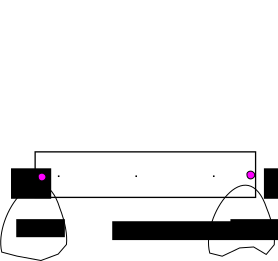
\includegraphics[scale=0.45]{./rep-landmarks.eps}
  %\vspace{-1ex}
  \caption{Using proxies for landmarks}
  \label{fig-angent-landmarks}
\end{minipage}
\begin{minipage}[b]{.24\textwidth}
  \centering
  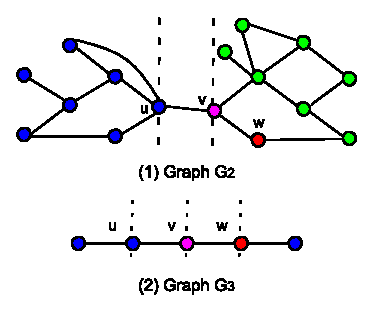
\includegraphics[scale=0.65]{./extended-proxies.eps}
  %\vspace{-1ex}
  \caption{Example proxies and \dras}
  \label{fig-proxies}
\end{minipage}%
\vspace{-4ex}
\end{figure}
}

\subsection{Routing Proxies and Deterministic Routing Areas}
\label{subsec-proxy-def}

We first present the notions of routing proxies and their deterministic routing areas.

\stitle{Proxies}. Given a node $u$ in graph $G(V, E)$, we say that $u$ is a {\em routing proxy} (or simply {\em proxy}) of a set of nodes, denoted by $A_{u}$, if and only if:

\sstab(1) node $u\in A_{u}$ is reachable to any node of $A_u$ in $G$,

\sstab(2) all neighbors of any node $v\in A_u\setminus \{u\}$ are in $A_u$,  and

\sstab(3) the size $|A_u|$ of $A_u$ is equal to or less than $c\cdot\lfloor\sqrt{|V|}\rfloor$, where $c$ is a small constant number, such as $2$ or $3$.


Here condition (1) guarantees the connectivity of subgraph $G[A_u]$,  condition (2) implies that not all neighbors of proxy $u$ are necessarily in $A_u$;
and condition (3), referred to as {\em size restriction}, limits the size of $A_u$ of proxy $u$.
Intuitively, one simply checks the graph by removing $u$ from $G$ and its newly created
\ccs , and a proxy of $u$ is a union of such \ccs whose total number of nodes is at most $c\cdot\lfloor\sqrt{|V|}\rfloor - 1$.




\stitle{Deterministic routing areas}. A node $u$ may be a proxy of multiple sets of nodes $A^1_u, \ldots, A^k_u$, and
we denote as $A^{+}_u$ the union of all the sets of nodes whose proxy is $u$ , \ie  $A^{+}_u$ = $A^1_u$ $\cup\ldots\cup$ $A^k_u$.

We refer to the {\em subgraph} $G[A^+_u]$ as a deterministic routing area (\dra) of proxy $u$.

Intuitively, \dra $G[A^+_u]$ is a {\em maximal} connected subgraph, union of a set of \ccs, that connects to the rest of graph $G$ through proxy $u$ only.
That is, for any node $v$ in $G[A^+_u]$ and any node $v$ in the rest of graph $G$, $u$ must appear on the shortest path $\path(v, v')$.

\stitle{Maximal proxies}.  We say that a proxy $u$ is {\em maximal} if there exist no other proxies $u'$ such that $u'\ne u$ and $A^+_{u} \subset A^+_{u'}$.

\stitle{Trivial proxies}. We say that a maximal proxy $u$ is {\em trivial} if $A^+_u$ contains itself only, \ie $A^+_{u}$ = $\{u\}$.


\stitle{Equivalent proxies}. We say that two proxies $u$ and $u'$ are {\em equivalent}, denoted by $u\equiv u'$, if $A^+_{u} = A^+_{u'}$.




We next illustrate these notions with an example below.

\begin{figure}
\centering
 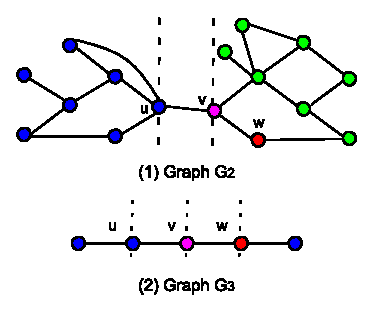
\includegraphics[scale=0.95]{./extended-proxies.eps}
 \vspace{-2ex}
 \caption{Example proxies and \dras}
  \label{fig-proxies}
\vspace{-3ex}
\end{figure}


\vspace{-0.5ex}
\begin{example}
\label{exm-proxies} First consider graph $G_2(V_2, E_2)$ in Fig.~\ref{fig-proxies}, and let $c\cdot\lfloor\sqrt{|V_2|}\rfloor$ =
$2\cdot\lfloor\sqrt{16}\rfloor$ = $8$, where $c = 2$ and $|V_2| = 16$.
\sstab(1) Node $u$ is a proxy, and its \dra is the subgraph in the left hand side of the vertical line across $u$;
\sstab(2) Node $v$ is a proxy, and its \dra is the subgraph in the left hand side of the vertical line across $v$;
\sstab(3) Node $w$ is not a proxy since it can not find a \dra with size less or equal than $8$;
\sstab(4)  Node $v$ is a maximal proxy, while node $u$ is not a maximal proxy since $A^+_u\subset A^+_v$.


We then consider graph $G_3(V_3, E_3)$ in Fig.~\ref{fig-proxies}, and let $c\cdot\lfloor\sqrt{|V_3|}\rfloor$ =
$2\cdot\lfloor\sqrt{5}\rfloor$ = $4$, where $c = 2$ and $|V_3| = 5$.
\sstab(1) Nodes $u, v$ and $w$ are three maximal proxies, whose \dras are all the entire graph $G_3$, and, hence,
\sstab(2) $u, v$ and $w$ are three equivalent proxies.
 \end{example}

\vspace{-1ex}
\stitle{Remark}. As illustrated by the above examples,  a \dra of graph $G(V, E)$ may have a size larger than $c\cdot\lfloor\sqrt{|V|}\rfloor$,
and multiple equivalent proxies.


We next first justify the necessity of introducing the size restriction for proxies.  Otherwise, \dras are simply \ccs, and are mostly useless.


\begin{prop}
\label{prop-proxy-cc} Without the size restriction, any node $u$ in a graph $G$ is a maximal proxy,
and its \dra $G[A^+_u]$ is exactly the connected component (\cc) to which $u$ belongs.
\end{prop}


We then show that proxies and \dras are {\em well defined}.


\begin{prop}
\label{prop-proxy-unique-dra} Any proxy in a graph has a unique \dra.
\end{prop}


\begin{prop}
\label{thm-proxy-disjoint} Given any two distinct proxies $u$ and $u'$, \\
(1) if $u\in A^+_{u'}$, then $A^+_{u}\subseteq A^+_{u'}$, \\
(2) if $u'\in A^+_{u}$, then $A^+_{u'}\subseteq A^+_{u}$,  and \\
(3) $A^+_{u}\cap A^+_{u'}$ = $\emptyset$, otherwise.
\end{prop}


By Proposition~\ref{thm-proxy-disjoint}, it is easy to have the following, which says when maximal proxies are concerned, there exists a unique set of non-overlapping \dras.

\begin{cor}
\label{cor-proxy-disjoint} Given any two maximal proxies $u$ and $u'$, then either $A^+_{u} = A^+_{u'}$ or $A^+_{u}\cap A^+_{u'}$ = $\emptyset$ holds.
\end{cor}


\vspace{-1ex}
\stitle{Remark}. Trivial proxies only represent themselves, and, hence, we are only interested in non-trivial maximal proxies (or simply called proxies) in the sequel.


\subsection{Properties of Proxies and DRAs}
\label{subsec-proxy-properties}

We next give an analysis of proxies and \dras, and show that they indeed hold good properties for answering shortest path and distance queries.
%



Indeed, the size restriction guarantees that the shortest distance computation within a \dra can be evaluated efficiently,
as shown below.


\begin{prop}
\label{pro-proxy-path} Given any two nodes $v, v'$ in the \dra $G[A^+_u]$ of proxy $u$ in graph $G$, \\
(1) the shortest path in $G[A^+_u]$ is exactly the one in the entire graph $G$, and\\
(2) it can be computed in linear time in the size of $G$.
\end{prop}


By Proposition~\ref{pro-proxy-path}, it is easy to derive the following.

\begin{cor}
\label{cor-proxy-distance} Given any two nodes $v, v'$ in the \dra $G[A^+_u]$ of proxy $u$ in graph $G$, \\
(1) the shortest distance $\dist(v, v')$ in $G[A^+_u]$ is exactly the one in the entire graph $G$, and\\
(2) it can be computed in linear time in the size of $G$.
\end{cor}


\begin{prop}
\label{pro-proxy-path-global} Given two nodes $v$ and $u$ with two distinct proxies $x$ and $y$, respectively, in graph $G$, the shortest path from $v$ to $u$ is $\path(v, x)/\path(x, y)/\path(y, u)$.
\end{prop}


Here $\path(v, x)/\path(x, y)/\path(y, u)$ is a path by concatenating paths $\path(v,x)$, $\path(x,y)$ and $\path(y,u)$.
By Proposition~\ref{pro-proxy-path-global}, it is easy to derive the following result.

\begin{cor}
\label{cor-proxy-distance-global} Given two nodes $v$ and $u$ with two distinct proxies $x$ and $y$, respectively, in graph $G$, the shortest distance $\dist(v, u)$ = $\dist(v, x)$ $+$ $\dist(x, y)$  $+$ $\dist(y, u)$.
\end{cor}


Propositions~\ref{pro-proxy-path},~\ref{pro-proxy-path-global} and Corollaries~\ref{cor-proxy-distance},~\ref{cor-proxy-distance-global} guarantee that the shortest paths and distances between the nodes in the \dras of two distinct proxies can be answered in a correct and efficient way.






\subsection{Query Answering with Routing Proxies}
\label{subsec-proxy-query}



\eat{%%%%%%%%
\begin{figure}[tb!]
%\vspace{-1ex}
\begin{center}
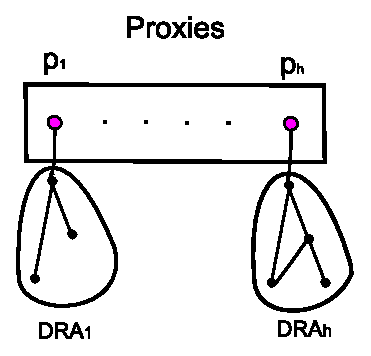
\includegraphics[scale=0.6]{./Proxy-framework.eps}
\end{center}
\vspace{-2ex}
\caption{Framework of using proxies}
\label{fig-angent-landmarks} \vspace{-2ex}
\end{figure}
}%%%%%%%%%%%%EAT

 Based on the above analyses, we present a framework for speeding-up shortest  path and distance query answering, which consists of two modules: {\em preprocessing} and {\em query answering}.
 %The framework for answering queries using proxies and \dras is illustrated in Fig.~\ref{fig-angent-landmarks}, in which each $p_i$ ($i\in[1, h]$) denotes a proxy, and is associated with its \dra.
 We next introduce the details of the framework.

\stitle{1. Preprocessing}. Given graph $G(V, E)$, the preprocessing module executes the following.

\sstab (1) It first computes all \dras and their maximal proxies with algorithm $\compDRAs$ (to be seen shortly in Section~\ref{sec-proxy-algorithms}).

\sstab (2) It then pre-computes and stores all the shortest paths and distances between any node in a \dra and its proxy.


\stitle{2. Query answering}. Given two nodes $s$ and $t$ in graph $G(V, E)$  and the pre-computed information, the query answering module executes the following.


\sstab (1) When nodes $s$ and $t$ belong to the same \dra $G[A^+_u]$ with proxy $u$ such that $A^+_u$ = $A^1_u\cup\ldots A^h_u$.

If $s$ and $t$ further fall into the same $A^i_u$ ($i\in[1,h]$), then it invokes the Dijkstra's algorithm on the subgraph $G[A^i_u]$ to compute the shortest path and distance between $s$ and $t$. Otherwise, it simply returns $\path(s, u)/\path(u, t)$ or $\dist(s, u)$ + $\dist(u, t)$, in constant time.

\sstab (2)  When $s$ and $t$ belong to two \dras $G[A^+_{u_s}]$ and $G[A^+_{u_t}]$ with proxies $u_s$ and $u_t$, respectively.

Observe that $\path(s, t)$ = $\path(s, u_s)/\path(u_s, u_t)/$ $\path(u_t, t)$ and $\dist(s, t)$ = $\dist(s, u_s)$ + $\dist(u_s, u_t)$ + $\dist(u_t, t)$, in which $\path(s, u_s)$, $\path(u_t, t)$, $\dist(s, u_s)$ and $\dist(u_t, t)$ are already known. Hence, it simply invokes an algorithm (\eg bidirectional Dijkstra~\cite{LubyR89}, \arcflag \cite{MohringSSWW05}, \ch~\cite{GeisbergerSSD08}, \tnr~\cite{bast2014route}) for computing $\path(u_s, u_t)$.
Similarly, the shortest distance $\dist(s, t)$ can be computed.

\stitle{Remarks}.
(1) To support shortest distance queries, for each node in a \dra, we store its corresponding proxy and the distance to the proxy. To support shortest path queries, we further keep the shortest paths from each proxy to all nodes in its \dra. Thus, we need $O(d)$ extra space to store the routing information to answer shortest path and distance queries, where $d$ is the total number of nodes in all \dras.

\sstab (2) Let $G'$ be the reduced subgraph of $G$ by removing all the nodes in \dras, but keeping their proxies, from graph $G$. It is easy to see that the main computation cost is reduced from $G$ to $G'$. As shown in the experimental study (Section~\ref{sec-expt}), on average about 1/3 nodes of a graph are captured by non-trivial proxies and their \dras, \ie $d$ is about $|V|/3$. That is, graph $G'$ is about 2/3 size of graph $G$, and hence our data reduction technique could reduce graph sizes and speed up shortest path and distance computations.

\subsection{Algorithm}

With emission probabilities and transition probabilities estimated from Equations
\ref{equ:emi-prob} and \ref{equ:trans-prob}, we can use the Viterbi algorithm to
compute the optimal path. The Viterbi algorithm is a dynamic programming
algorithm that can quickly detect a sequence of states that maximizes the joint
probability, which is the product of the emission probabilities and transition
probabilities of all the states in the sequence. The detected sequence is the
path with maximum likelihood and thus the global optimal path.



\begin{large}
\begin{algorithm}
\caption{The CT-MM Algorithm}\label{alg:viterbi}
\small
\begin{algorithmic}[1]
 \State  \textbf{Input}: $\overline{\mathcal{T}}$,$\epsilon$,G(V,E)
 \State  \textbf{Output}: map matching result R

 \State $E_1 \gets findCand(G(V,E),p_1)$.

 \State \textbf{Initialize} $f[r_1^k] = p(r_{1}^k|p_{1}), k = 1,2,\cdots,10$.

 % \For{each line segments in $\overline{\mathcal{T}}$}
 \For{$i = 2 \to n$}
   % \State extract candidate set of that GPS point from road network.
   \State $P_i \gets \overline{\mathcal{T}}[i].e$
   \State $P_{i-1} \gets \overline{\mathcal{T}}[i].s$
   \State $E_i \gets findCand(G(V,E),P_i)$.\Comment{find candidate set}
   % \State extract subgraph between the previous and current GPS point.
   \State $G_s \gets extract(G(V,E),\overline{\mathcal{T}}[i],\epsilon)$.
   \Comment{extract subgraph}
   \For{$r_i^j \in E_i$}
      \State compute $p(r_{i}^j|P_{i})$ by equation (6)
      \State $f[r_{i}^j] = -\infty$
      \For{$r_{i-1}^k \in E_{i-1}$}
      % \State compute shortest path from $r_{i-1}$ to $r_{i})$ in the sub action graph.
      % \State $sp_i^j\gets shortestPath(r_{i-1},r_{i},sbGraph)$
      \State $R_{j,k} \gets PathRec(G_s,r_i^j,r_{i-1}^k)$.\Comment{path recovery}
      \State compute $p(r_{i-1}^k,r_{i}^j)$ by equation (7)
      \State $Conj\gets f[r_{i-1}^j] * p(r_{i-1}^j,r_{i}^k) * p(r_{i}^j|P_{i})$
      \If{$Conj \ge f[r_{i}^k]$}
        \State $f[r_{i}^k] = Conj$
        \State $Pre[r_{i}^k] = r_{i-1}^j$
      \EndIf
    \EndFor
  \EndFor
  \EndFor
  \State $R = \argmax_{r_1^{k_1}\rightarrow r_2^{k_2}\rightarrow \cdots \rightarrow r_n^{k_n}}f[r_{n}^{k_n}]$
\State \textbf{return} $R$\Comment{The matched result is R}

% \Procedure{getSubGraph}{$p_{i-1},p_i,length,width$}
% \State get bounding box.
% \EndProcedure
\end{algorithmic}
\end{algorithm}
\end{large}


\section{Query Answering with Routing Proxies}
\label{sec-query}

In this section, we show how to answer shortest path and distance queries using routing proxies.

\eat{%%%%%%%%
\begin{figure}[tb!]
%\vspace{-1ex}
\begin{center}
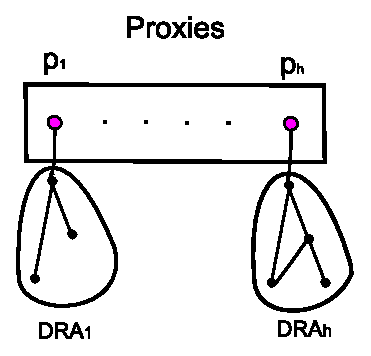
\includegraphics[scale=0.6]{./Proxy-framework.eps}
\end{center}
\vspace{-2ex}
\caption{Framework of using proxies}
\label{fig-angent-landmarks} \vspace{-2ex}
\end{figure}
}%%%%%%%%%%%%EAT

 Based on the previous analyses, we present a framework for speeding-up shortest  path and distance query answering, which consists of two modules: {\em preprocessing} and {\em query answering}.
 %The framework for answering queries using proxies and \dras is illustrated in Fig.~\ref{fig-angent-landmarks}, in which each $p_i$ ($i\in[1, h]$) denotes a proxy, and is associated with its \dra.
 We next introduce the details of the framework.

\stitle{1. Preprocessing}. Given graph $G(V, E)$, the preprocessing module executes the following.

\sstab (1) It first computes all \dras and their maximal proxies with algorithm $\compDRAs$ (to be seen shortly in Section~\ref{sec-proxy-algorithms}).

\sstab (2) It then pre-computes and stores all the shortest paths and distances between any node in a \dra and its proxy.

To support shortest distance queries, for each node in a \dra, we store its proxy $u$, its distance to $u$ and the component of $A^{+}_u$ to which it belongs,
and, moreover, to support shortest path queries, we further keep the shortest paths from proxy $u$ to all nodes in the \dra.

\sstab (3) It finally computes the reduced subgraph $G'$ by removing all \dras, but keeping their proxies, from graph $G$. 


\stitle{2. Query answering}. Given two nodes $s$ and $t$ in graph $G(V, E)$  and the pre-computed information, the query answering module executes the following.


\sstab (1) When nodes $s$ and $t$ belong to the same \dra $G[A^+_u]$ with proxy $u$ such that $A^+_u$ = $A^1_u\cup\ldots A^h_u$.

If $s$ and $t$ further fall into the same component $A^i_u$ ($i\in[1,h]$), it invokes the Dijkstra's algorithm on the subgraph $G[A^i_u]$ to compute the shortest path and distance between $s$ and $t$. Otherwise, it simply returns $\path(s, u)/\path(u, t)$ or $\dist(s, u)$ + $\dist(u, t)$ in constant time.

\sstab (2)  When $s$ and $t$ belong to two \dras $G[A^+_{u_s}]$ and $G[A^+_{u_t}]$ with proxies $u_s$ and $u_t$, respectively.

By the analyses in Section~\ref{subsec-proxy-properties}, we know that $\path(s, t)$ = $\path(s, u_s)/\path(u_s, u_t)/$ $\path(u_t, t)$, in which $\path(s, u_s)$ and $\path(u_t, t)$ are already known. Hence, it simply invokes an algorithm (\eg bidirectional Dijkstra~\cite{LubyR89}, \arcflag \cite{MohringSSWW05}, \ch~\cite{GeisbergerSSD08}, \tnr~\cite{bast2014route}, \ah~\cite{zhu2013shortest}) on the reduced graph $G'$ for computing $\path(u_s, u_t)$.

Similarly, the shortest distance $\dist(s, t)$ = $\dist(s, u_s)$ + $\dist(u_s, u_t)$ + $\dist(u_t, t)$ can be computed.

We next illustrate how shortest path and distance queries are performed  with an example below.


%%%%%%%%%%%%%%%%%%%%%%%%%%%%%%%%%%%%%%%%%%%%%%%%%%
\begin{figure}[tb!]
%\vspace{-1ex}
\begin{center}
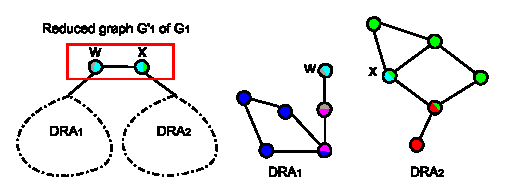
\includegraphics[scale=0.95]{./Example-framework.eps}
\end{center}
\vspace{-2ex}
\caption{Example query answering}
  \label{fig-query-answering}\vspace{-3ex}
\end{figure}

\begin{example}
\label{exm-query}
Consider graph $G_1$ and its \bccs in Fig.~\ref{fig-cut-nodes}(1), in which the \dras and their maximal proxies are computed by algorithm $\compDRAs$, \ie\ $\dra_1$ = $\{u, v, BC_1, BC_2, BC_3\}$ with its proxy $w$ and $\dra_2$ = $\{y, BC_5, BC_6\}$ with its proxy $x$, as shown in Fig.~\ref{fig-query-answering}. Note that here both $A^{+}_w$ and $A^{+}_x$ have single components. Moreover, the reduced graph $G'_1$ of $G_1$  is the subgraph with nodes $w$ and $x$ only.




\sstab(1) Consider nodes $s$ in $\dra_1$  and $t$ in $\dra_2$, we first compute $\dist(w, x)$ or $\path(w,x)$ on $G'_1$, and then 
let $\dist(s, t)$ = $\dist(s, w)$ + $\dist(w, x)$ + $\dist(x, t)$ or $\path(s, t)$ = $\path(s, w)/\path(w, x)/\path(x, t)$.
Note that here $\dist(s, w)$, $\dist(x, t)$, $\path(s, w)$ and $\path(x, t)$ have all been computed in the precessing stage.


\sstab(2) If nodes $s$ and $t$ are both in $\dra_1$  or $\dra_2$, we directly compute their shortest path or distance on  $\dra_1$  or $\dra_2$,
as they have single components.
\end{example}

\vspace{-1ex}
\stitle{Remarks}.
(1) As shown above, we need $O(d)$ extra space to store the routing information to compute shortest paths and distances, where $d$ is the total number of nodes in all \dras.

\sstab (2) It is easy to see that the main computation cost is reduced from graph $G$ to its reduced graph $G'$. As shown in the experimental study (Section~\ref{sec-expt}), on average about 1/3 nodes of a graph are captured by non-trivial proxies and their \dras, \ie $d$ is about $|V|/3$. That is, the reduced graph $G'$ is about 2/3 size of the original graph $G$, and hence our data reduction technique could reduce graph sizes and speed up shortest path and distance computations. 
\section{Experimental Study}
\label{sec-expt}

%%%%%%%%%%%%%%%%%%%%%%%%%%%%%%%%%%%%%%%%%%%%%%%%%%

%We next present an experimental study to show how proxies speed up shortest  path and distance queries.
%Using real-life networks, we conducted three
%sets of experiments to evaluate:
%(1) the performance of proxies,
%(2) the efficiency of (bidirectional) Dijkstra~\cite{LubyR89}, \arcflag \cite{MohringSSWW05}, \tnr \cite{arz2013transit} and their counterparts with proxies (Proxy+Dijkstra, Proxy+\arcflag, Proxy+\tnr) with respect to  graph queries, and (3) the efficiency of these algorithms with respect to graph sizes.
Using real-life road networks and social graphs, we next conduct an extensive experimental study to evaluate: (1) the performance of computing routing proxies, and (2) how routing proxies speed up shortest  path and distance queries, by comparing the efficiency of (bidirectional) Dijkstra~\cite{LubyR89}, \arcflag \cite{MohringSSWW05}, \tnr \cite{arz2013transit}, \ah \cite{zhu2013shortest} with their counterparts using proxies (Proxy+Dijkstra, Proxy+\arcflag, Proxy+\tnr, Proxy+\ah) with respect to graph queries and graph sizes.

\eat{%%%%%%%%%%%%EAT
\begin{table}[t!]
\label{tab-datasets}
\caption{Real-world graphs}
\vspace{-1ex}
\begin{center}
%\begin{small}
\begin{tabular}{|c|c|r|r|}
\hline
Name                            &  Regions               & \# of Nodes  &  \# of Edges \\
\hline\hline
DBLP14    &   A subgraph of DBLP                 & 141,359  &   246,462 \\ \hline
DBLP    & DBLP & 317,080 & 1,049,866 \\ \hline
CO      &  Colorado              & 435,666      &  521,200  \\ \hline
FL      &  Florida               & 1,070,376    &  1,343,951  \\ \hline
CA      &  California \& Nevada   & 1,890,815   &  2,315,222  \\ \hline
E-US    &  Eastern US            & 3,598,623    &  4,354,029 \\ \hline
W-US    &  Western US            & 6,262,104    &  7,559,642  \\ \hline
C-US    &  Central US            & 14,081,816   &  16,933,413 \\ \hline
US      &  Entire US             & 23,947,347   &  28,854,312  \\ \hline
\end{tabular}
%\end{small}
\end{center}
\end{table}
}%%%EAT%%%%%%%%%%%%%%%%%%%%%%%%%%%%%%%%%%%%%%%%%%%%%%%

\begin{table*}[t!]
\label{tab-exp1-proxies-dras}
\begin{center}
\begin{scriptsize}
\caption{Effectiveness of proxies and \dras}
\vspace{-2ex}
\begin{tabular}{|c||c|c|c||r|r|r|r|r|r|}
\hline
  \multicolumn{4}{|c||}{\bf Datasets} & \multicolumn{6}{c|}{\bf Evaluation of Computing Routing Proxies}\\
  \hline
                          &  &  &  &  \multicolumn{1}{c|}{\bf Proxies}   &  \multicolumn{1}{c|}{\bf Nodes in \dras}  & \multicolumn{1}{c|}{\bf Extra space} & \multicolumn{1}{c|}{\bf Space of $G$} & \multicolumn{1}{c|}{\bf Space of $G'$} & \multicolumn{1}{c|}{\bf Time}\\

  \raisebox{1.5ex}[0pt]{\bf Graphs $G$} &   \raisebox{1.5ex}[0pt]{\bf Regions} &   \raisebox{1.5ex}[0pt]{\bf \# of Nodes} &   \raisebox{1.5ex}[0pt]{\bf \# of Edges} & \multicolumn{1}{c|}{\bf (\#, \%)}  &  \multicolumn{1}{c|}{\bf (\#, \%)}  & \multicolumn{1}{c|}{\bf (MB)} & \multicolumn{1}{c|}{\bf (MB)} & \multicolumn{1}{c|}{\bf (MB)} & \multicolumn{1}{c|}{\bf (Sec.)}\\
\hline\hline
DBLP14      &   Subgraph of DBLP          & 141,359  &   246,462     &  (14, 090, 9.8)         & (102,085, 72.2)  & 1.56 & 4.30 & 1.36 &  1.5 \\ \hline
DBLP        & DBLP                        & 317,080 & 1,049,866     & (31,475 , 9.9)             & (105,671 , 33.3) & 1.61 & 17.22 & 14.29  & 5.7 \\ \hline
CO          &  Colorado              & 435,666      &  521,200       &  (56,277, 12.9)         & (156,329, 35.9)  & 2.38  & 9.61 & 6.64 & 3.47  \\ \hline
FL          &  Florida               & 1,070,376    &  1,343,951      &  (140,382, 13.1)        & (378,804, 35.4)  & 5.78  & 24.59 & 17.12 &  9.9 \\ \hline
CA          &  California \& Nevada   & 1,890,815   &  2,315,222      &  (273,191, 14.4)        & (623,811, 33.0)  & 9.52  & 42.55 & 30.66 & 21.1 \\ \hline
E-US        &  Eastern US            & 3,598,623    &  4,354,029    &  (546,481, 15.2)        & (1,228,876, 34.1)& 18.75  & 80.17 & 56.48 &  52.5  \\ \hline
W-US        &  Western US            & 6,262,104    &  7,559,642      &  (869,907, 13.9)        & (2,116,382, 33.8)& 32.29  & 139.23 & 98.68 &  111.9 \\ \hline
C-US        &  Central US            & 14,081,816   &  16,933,413    &  (2,034,358, 14.4)      & (4,583,413, 32.5)& 69.94 & 312.09 & 225.28 & 435.8 \\ \hline
US          &  Entire US             & 23,947,347   &  28,854,312      &  (3,452,222, 14.4)      & (7,927,453, 33.1)& 120.96 & 531.63 & 380.59 &  1,925.4 \\ \hline
\end{tabular}
\end{scriptsize}
\end{center}
\vspace{-4ex}
\end{table*}
%%%%%%%%%%%%%%%%%%%





\subsection{Experimental Settings}
We first introduce the settings of our experimental study.







\stitle{Real-life graphs}.
We use two types of datasets, and the details of all datasets are reported in Table~1.



\sstab (1) The first type of datasets is {\em co-authorship networks}. We extracted co-authorship graphs from DLBP~\cite{snapnets}, where each node in the graph represents an author and two authors are connected if they have published papers together. The edge weight is computed by a revised Adamic/Adar similarity function: $w(u,v) = \frac{1}{\sum_{z\in {\Gamma(u)\cap \Gamma(v) \cup \{u,v\}}}\frac{1}{\log{|\Gamma(z)|}}}$, where $\Gamma(u)$ and $\Gamma(v)$ are the sets of neighbors of nodes $u$ and $v$, respectively. The weight of the edge $(u,v)$ represents the closeness between $u$ and $v$ and a smaller weight means the two authors are closer. \tnr is designed for road networks and it is very inefficient for \tnr to preprocess dense graphs such as DBLP (it took more than 1 week to finish the preprocessing). To guarantee that we can evaluate the improvement of \tnr with proxies on general graphs, we remove all nodes whose degrees are higher than 14, and choose the largest connected component in the remaining graph, referred to as \dblpone.


\sstab (2) The second type of datasets is {\em road networks}. We chose seven standard road network datasets of various sizes from the Ninth DIMACS
Implementation Challenge~\cite{dimacs-datasets} (available at {\url{http://www.dis.uniroma1.it/challenge9/download.shtml}}). Each road network is released as an undirected graph representing a part of the road network in the United States, where each edge weight is the distance (an integer) required to travel between the two endpoints of the edge.


\stitle{Shortest  path and distance queries}. Our queries were generated as follows.
(1) On each road  or co-authorship network, we first randomly choose a node $u$, and run a Dijikstra algorithm from $u$ to find the node $s$ that is farthest from $u$. Then we run a Dijkstra again from $s$ to find the node $t$ that is farthest from $s$. Let $\ell$ be the distance $\dist(s,t)$ from $s$ to $t$.
(2) We then randomly chose ten thousand node pairs from
the road network to compose $Q_i (i \in [1,7])$, such that the grid
distance of all node pairs in $Q_i$ is in $[2^{i-9}\cdot\ell, 2^{i-8}\cdot\ell)$.
For each query set $Q_i$ $(i\in [1,7])$, we report the average running time of 10,000 queries in the set.

%On each road network, we generated eight sets $Q_1$, $Q_2$, $\dots$ , $Q_{7}$ of
%queries. (1) We first imposed a $256 \times 256$ grid on the
%road network and computed the side length $\ell$ of each grid cell.
%(2) We then randomly chose ten thousand node pairs from
%the road network to compose $Q_i (i \in [1, 7])$, such that the grid
%distance of all node pairs in $Q_i$ is in $[2^{i-1}\cdot\ell, 2^i\cdot\ell)$. Note
%that the grid distance of two nodes $u, v$ in a query set is the distance of the cells into which $u$ and $v$ fall, respectively.
%Moreover, the grid distance of any node pair in $Q_i$ is
%larger than the grid distance of all node pairs in $Q_{i-1}$.
%For each query set $Q_i$ $(i \in [1, 7])$, we report the average running time of 10,000 queries in the set.

\stitle{Algorithms.} We implemented algorithms bidirectional-Dijkstra~\cite{LubyR89}, \arcflag~\cite{MohringSSWW05}, \tnr~\cite{arz2013transit} and \ah \cite{zhu2013shortest}.

For \arcflag, it first needs to partition graphs to pre-compute information on whether an arc is useful for a shortest path search. Any possible partition methods~\cite{kl70,Karypis98,YangYZK12, delling2011graph} can be used here. Since we have both road networks and co-authorship networks, we adopted the latest version 5.0.2 of \metis~\cite{metis}, implemented with ANSI C, because it is open source and performs quite well in practice.

For \tnr, since we do not have coordinates information in the co-authorship network, we implemented the CH-based \tnr~\cite{arz2013transit} that does not require the geometry information.

We obtained the C++ implementation of \ah from \cite{zhu2013shortest} and adopted its default settings.



\stitle{Implementations.} All algorithms were implemented with C++, and
all experiments were run on a PC with an Intel Xeon(R) X5650 CPU@2.67GHz
and 24GB of memory.






%\subsection{Experimental Results}
%We next present our findings. In all experiments, we tested the datasets in Table~1, and fixed the constant $c = 2$ for computing proxies on all graphs.
%The preprocessing of \arcflag was slow, and it spent over four days on C-US. Hence, we did not test the largest dataset US for \arcflag.
\subsection{Performance of Computing Routing Proxies}
Using the datasets in Table~1, we first conduct experiments to evaluate the performance of computing proxies, \ie\ how many nodes can be represented by proxies, how much extra space we need to store the routing information for the proxies, and how much time we need to find all proxies. More specifically, we evaluate (1) the number of non-trivial proxies, (2) the number and percentage of the nodes represented by the proxies (excluding the proxies themselves from \dras), (3) the extra space cost of using proxies, (4) the space overhead of storing the original graph $G$, (5) the space overhead of storing the reduced graph $G'$, and (6) the efficiency of algorithm $\compDRAs$ for computing proxies and their \dras. We fixed the constant $c = 2$ for computing proxies on all graphs. When computing the space overhead for the original graphs and the reduced graphs, we assume that all graphs are stored as adjacency lists. The experimental results are reported in Table~1.

%Note that to speed up shortest  path and distance queries, for each node represented by a proxy, we need to store (1) the distance between the node and its proxy, and (2) the shortest path from the node to its proxy. Distances are stored as 4-byte integers and it takes $4 \cdot |V_{\dras}|$ bytes to store all the distances, where $V_{\dras}$ is the set of nodes in all \dras. All the shortest paths between the nodes in a \dra and its proxy form a tree whose root is the proxy. Each node is also represented as a 4-byte integer. So it takes $ 4 \cdot (|V_{proxy}|+ |V_{\dras}|) $ bytes to maintain all the trees, where $V_{proxy}$ is the set of proxies. So the extra space cost of using proxies is $4 \cdot |V_{proxy}| + 8 \cdot |V_{\dras}|$ bytes. The results are reported in Table~2.
\stitle{1. Effectiveness evaluation}.
For the \dblp graph, about $1/10$ nodes are non-trivial proxies, and about $1/3$ nodes are captured by proxies in the graph, which means basically the reduced graph is only about $2/3$ of the original input graph. For the \dblpone graph, about $1/10$ nodes are non-trivial proxies, and about $2/3$ nodes are captured by the \dras of proxies in the graph, which means basically the reduced graph is only about $1/3$ of the original input graph.

For all the road graphs,  about $1/7$ nodes are non-trivial proxies, and about $1/3$ nodes are captured by the \dras of these proxies, which means basically the reduced graph is only about $2/3$ of the original input graph.

 Moreover, although the size restriction is $\le 2\cdot\lfloor\sqrt{|V|}\rfloor$, \dras are typically small such that each proxy represents 2 or 3 other nodes on average.


\begin{figure*}[t!]
%\vspace{-1ex}
\begin{center}
\hspace{-4ex}
\subfigure[{\scriptsize DBLP14}]{\label{fig-dist-dj-varyQ-dblp}
\includegraphics[scale=0.45]{./exp/query_dblp_dist_dj.eps}}
\hspace{-4ex}\vspace{-1.5ex}
\subfigure[{\scriptsize CA}]{\label{fig-dist-dj-varyQ-CAL}
\includegraphics[scale=0.45]{./exp/query_cal_dist_dj.eps}}
\hspace{-4ex}\vspace{-1.5ex}
\subfigure[{\scriptsize E-US}]{\label{fig-dist-dj-varyQ-E-US}
\includegraphics[scale=0.45]{./exp/query_eus_dist_dj.eps}}
\hspace{-4ex}\vspace{-1.5ex}
\subfigure[{\scriptsize C-US}]{\label{fig-dist-dj-varyQ-C-US}
\includegraphics[scale=0.45]{./exp/query_cus_dist_dj.eps}}
\end{center}
\vspace{1ex}
\caption{Varying graph queries  for shortest distances: Dijkstra vs. Proxy+Dijkstra}
\label{fig:performance_dist_queries_dj}
\vspace{-1ex}
\end{figure*}

\begin{figure*}[t!]
%\vspace{-2ex}
\begin{center}
\hspace{-4ex}
\subfigure[{\scriptsize DBLP14}]{\label{fig-dist-af-varyQ-dblp}
\includegraphics[scale=0.45]{./exp/query_dblp_dist_af.eps}}
\hspace{-4ex}\vspace{-1.5ex}
\subfigure[{\scriptsize CA}]{\label{fig-dist-af-varyQ-CAL}
\includegraphics[scale=0.45]{./exp/query_cal_dist_af.eps}}
\hspace{-4ex}\vspace{-1.5ex}
\subfigure[{\scriptsize E-US}]{\label{fig-dist-af-varyQ-E-US}
\includegraphics[scale=0.45]{./exp/query_eus_dist_af.eps}}
\hspace{-4ex}\vspace{-1.5ex}
\subfigure[{\scriptsize C-US}]{\label{fig-dist-af-varyQ-C-US}
\includegraphics[scale=0.45]{./exp/query_cus_dist_af.eps}}
\end{center}
\vspace{1ex}
\caption{Varying graph queries  for shortest distances: \arcflag vs. Proxy+\arcflag}
\label{fig:performance_dist_queries_af}
\vspace{-1ex}
\end{figure*}


\begin{figure*}[t!]
%\vspace{-2ex}
\begin{center}
\hspace{-4ex}
\subfigure[{\scriptsize DBLP14}]{\label{fig-dist-tnr-varyQ-dblp}
\includegraphics[scale=0.45]{./exp/query_dblp_dist_tnr.eps}}
\hspace{-4ex}\vspace{-1.5ex}
\subfigure[{\scriptsize CA}]{\label{fig-dist-tnr-varyQ-CAL}
\includegraphics[scale=0.45]{./exp/query_cal_dist_tnr.eps}}
\hspace{-4ex}\vspace{-1.5ex}
\subfigure[{\scriptsize E-US}]{\label{fig-dist-tnr-varyQ-E-US}
\includegraphics[scale=0.45]{./exp/query_eus_dist_tnr.eps}}
\hspace{-4ex}\vspace{-1.5ex}
\subfigure[{\scriptsize C-US}]{\label{fig-dist-tnr-varyQ-ME-C-US}
\includegraphics[scale=0.45]{./exp/query_cus_dist_tnr.eps}}
\end{center}
\vspace{1ex}
\caption{Varying graph queries  for shortest distances: \tnr and Proxy+\tnr}
\label{fig:performance_dist_queries_tnr}
\vspace{-1ex}
\end{figure*}

\begin{figure*}[t!]
%\vspace{-2ex}
\begin{center}
\hspace{-4ex}
\subfigure[{\scriptsize CA}]{\label{fig-dist-ah-varyQ-CAL}
\includegraphics[scale=0.45]{./exp/query_cal_dist_ah.eps}}
\hspace{-4ex}\vspace{-1.5ex}
\subfigure[{\scriptsize E-US}]{\label{fig-dist-ah-varyQ-E-US}
\includegraphics[scale=0.45]{./exp/query_eus_dist_ah.eps}}
\hspace{-4ex}\vspace{-1.5ex}
\subfigure[{\scriptsize C-US}]{\label{fig-dist-ah-varyQ-ME-C-US}
\includegraphics[scale=0.45]{./exp/query_cus_dist_ah.eps}}
\end{center}
%\vspace{1ex}
\caption{Varying graph queries  for shortest distances: \ah vs. Proxy+\ah}
\hrule
\label{fig:performance_dist_queries_ah}
\vspace{-2ex}
\end{figure*}




\stitle{2. Efficiency evaluation}.
In the \dblp graph, proxies can be found in about 6 seconds. In the \dblpone graph, it only takes 1.5 seconds to find all \dras with their proxies.

In all road networks, proxies can be found efficiently. Algorithm $\compDRAs$ also scales well, and it can be done in less than half an hour for the largest graph US with $2.4$ $\times$ $10^7$ nodes and $5.7$ $\times$ $10^7$ edges.

\stitle{3. Space evaluation}.
To support shortest distance queries, for each node in a \dra, we store its proxy $u$, its distance to $u$ and the component of $A^{+}_u$ to which it belongs, and, moreover, to support shortest path queries, we further keep the shortest paths from proxy $u$ to all nodes in the \dra. Assume that distances are stored as a 4-byte integer. Each node is represented as a 4-byte integer. Then the extra space that we need for shortest path and distance queries is $16\cdot |V_{dra}|$, where $V_{dra}$ is the set of nodes in all \dras.

In the \dblp and \dblpone graphs, it only takes about 1.6 MB extra space to store the routing information for all proxies, since there are similar number of nodes in the \dras of both datasets. Observe that by using proxies to represent all nodes in \dras, the reduced graph  has a smaller size than the original graph, especially for the \dblpone graph. In the \dblpone graph, 72.2\% of its nodes are captured by proxies, which leads to a much smaller reduced graph.

In all road networks, it incurs small extra space overhead to store the routing information for proxies. Only about 100 MB extra space is taken for the largest graph US. The use of proxies also results in a smaller reduced graph. As shown in Table~1, the size of the reduced graph is about 70\% of the original graph on average.



From these tests, we can find that using proxies is a light-weight optimization technique, which scales well to large networks, and incurs appropriate space overhead. %These properties benefit existing shortest  path and distance algorithms, such as (bidirectional) Dijkstra, \arcflag , \tnr and \ah, to be seen immediately.

\subsection{Benefits of Using Routing Proxies}
Our proxies can be used as a preprocessing step before we apply other existing approaches.
We next conduct experiments to show the comparison results of an existing approach (\ie \ Dijkstra, \arcflag, \tnr and \ah) with its counterpart using proxies, using the datasets in Table~1.



Due to the space limitation, we sometimes only report the results on \dblpone, CA, E-US, and C-US.
%A more detailed results can be found in the supplementary document.
We fixed the constant $c = 2$ for computing proxies on all graphs. Note that \ah requires the coordinate information to answer shortest path or distance queries, which is not available in \dblp and \dblpone. Thus, we only report results on CA, E-US, and C-US for \ah and its counterpart.
%The preprocessing of \arcflag was slow, and it spent over 4 days on C-US. Hence, we did not test the largest road network dataset US for \arcflag.
%\tnr invokes Contract Hierarchies (\ch) for preprocessing and \ch is very inefficient on dense graphs. Unfortunately \dblp is a very dense graph and it took more than 7 days for \ch to finish preprocessing on \dblp. Thus we tested \dblpone, instead of \dblp, for the performance of shortest path and distance queries. The CH-based \tnr whose space cost was very high, and consequently, and we could not run either \tnr or Proxy+\tnr on the largest road network dataset US, as both of them ran out of memory. Hence, we did not test the largest graph for \tnr as well. However, on the second largest road network dataset C-US, Proxy+\tnr can while \tnr cannot. We report this to show that proxies serve as a data reduction technique and benefit existing methods in terms of space cost as well.




\stitle{1. Effectiveness  \wrt graph queries}.
%In the second set of experiments, we justified that the \gdp problem could be solved well by \metis, originally for traditional graph partitioning problems. Using the shrink graphs generated at Exp-1, we evaluated the effectiveness and  efficiency of \metis. To ensure the query efficiency of \disland, each fragment has at most $c \cdot \lfloor\sqrt{|V|}\rfloor$ number of nodes. We used the multilevel bisection method of \metis with the balance factor fixed to 1.003. The results are reported in Table~4.
%
In this set of experiments, we evaluated the efficiency of shortest path and distance queries with respect to the graph queries.

For the \arcflag and Proxy+\arcflag methods, the graph and the reduced graph are partitioned into fragments such that each fragment has at most $2\cdot \lfloor\sqrt{|V|}\rfloor$ nodes in order to add labels to edges. We used \metis to partition graphs with the balance factor fixed to 1.003.

For the \tnr and Proxy+\tnr methods, we always select 10,000 transit nodes, as suggested in \cite{arz2013transit}. Note that the space cost of the CH-based \tnr is very high. Consequently, we could not run \tnr on C-US as it ran out of memory. However, we can successfully run Proxy+\tnr on C-US. We report this to show that proxies serve as a data reduction technique and benefit existing methods in terms of space cost as well. \tnr invokes Contract Hierarchies (\ch) \cite{GeisbergerSSD08} to preprocess the graph and \ch runs very slowly on \dblp (it took more than 7 days to run \ch on \dblp). Thus we report the results on \dblpone and all the road networks.

The results of distance queries and path queries are reported in Figures~\ref{fig:performance_dist_queries_dj} and \ref{fig:performance_path_queries_dj} (comparison between Dijkstra and Proxy+Dijkstra), Figures~\ref{fig:performance_dist_queries_af} and~\ref{fig:performance_path_queries_af} (comparison between \arcflag and Proxy+\arcflag), Figures~\ref{fig:performance_dist_queries_tnr} and~\ref{fig:performance_path_queries_tnr} (comparison between \tnr and Proxy+\tnr), and Figures~\ref{fig:performance_dist_queries_ah} and~\ref{fig:performance_path_queries_ah} (comparison between \ah and Proxy+\ah), respectively.

In the co-authorship network \dblpone, the results show that with the help of proxies, Proxy+Dijkstra, Proxy+\arcflag and Proxy+\tnr all achieve a better performance than their counterparts Dijkstra, \arcflag and \tnr without proxies, respectively. On average, the time cost of Proxy+\arcflag, Proxy+Dijkstra and Proxy+\tnr is about 96\%, 51\% and 51\% of their counterparts without proxies for distance queries, and 98\%, 49\% and 76\% of their counterparts without proxies for shortest path queries, respectively. More specifically, we can see that (1) proxies have a better speed-up effect on bidirectional Dijkstra and \tnr than \arcflag, (2) for \arcflag, proxies have a better speed-up effect when the two query nodes are far from each other, which is different from the observation on road networks. To explain the second observation, we need to notice that about 2/3 nodes are captured by proxies in \dblpone. Thus two close nodes are more likely to fall into the same \dras. Since there are no speed-up techniques used inside single \dras, the search space saved by proxies is less than using \arcflag alone.

In the road networks, the results show that with the help of proxies, Proxy+Dijkstra and Proxy+\arcflag can achieve a better performance than their counterparts without proxies, respectively. On average, the time cost of Proxy+\arcflag, Proxy+Dijkstra and Proxy+\ah is about 80\%, 68\% and 99\% of their counterparts without proxies for distance queries, and 82\%, 67\% and 99\% of their counterparts without proxies for shortest path queries, respectively. More specifically, we can see that (1) proxies have a better speed-up effect on bidirectional Dijkstra than \arcflag, (2) for \arcflag, proxies have a better speed-up effect when the two query nodes are close to each other, (3) different from \arcflag, proxy+Dijkstra has a better performance when the query nodes are far from each other, and (4) though \ah is one of the state-of-art method for shortest path and distance queries, proxies still improves the its efficiency about 1\%. To explain these observations, we need to think how much search space is saved by proxies. Since \arcflag has already used flags on edges to reduce the search space, the proportion of search space saved by proxies is smaller than bidirectional Dijkstra. That explains why proxies have a better speed-up effect on bidirectional Dijkstra. For \arcflag, two close nodes are more likely to fall into the same partition. In this case, the effect of flags on edges is less useful and the search space saved by proxies takes a large proportion, which explains the second observation. For bidirectional Dijkstra, proxies can save more search space when the query nodes are far from each other. As a state-of-art approach for shortest path and distance queries, the search space of \ah is much smaller than Dijkstra and \arcflag. However, the search space of \ah is still reduced, and \ah still benefits from proxies in terms of efficiency.

Proxy+\tnr achieves a comparable performance to its counterpart without proxies. This is because for \tnr, a heuristic method is used to generate the node order, based on the structure of the graph. And the node order can affect the performance of \tnr. Since we reduce the input graph by using proxies, the reduced graph has a different topology structure. Thus a different node order will be generated. So it is hard to guarantee that Proxy+\tnr outperforms \tnr. We should also notice that \tnr cannot run on C-US while Proxy+\tnr can. To explain this, we first recall that for \tnr, we have to store the access nodes and distances for each node. For the original input of C-US, there are too many nodes and it runs out of memory. By using proxies, about 1/3 nodes are captured by proxies and we only need to run \tnr on 2/3 of the input graph, which is more practical.


\begin{figure*}[t!]
%\vspace{-1ex}
\begin{center}
\hspace{-4ex}
\subfigure[{\scriptsize DBLP14}]{\label{fig-path-dj-varyQ-dblp}
\includegraphics[scale=0.45]{./exp/query_dblp_path_dj.eps}}
\hspace{-4ex}\vspace{-1.5ex}
\subfigure[{\scriptsize CA}]{\label{fig-path-dj-varyQ-CAL}
\includegraphics[scale=0.45]{./exp/query_cal_path_dj.eps}}
\hspace{-4ex}\vspace{-1.5ex}
\subfigure[{\scriptsize E-US}]{\label{fig-path-dj-varyQ-E-US}
\includegraphics[scale=0.45]{./exp/query_eus_path_dj.eps}}
\hspace{-4ex}\vspace{-1.5ex}
\subfigure[{\scriptsize C-US}]{\label{fig-path-dj-varyQ-C-US}
\includegraphics[scale=0.45]{./exp/query_cus_path_dj.eps}}
%\hfill
%\vspace{-1ex}
\end{center}
\vspace{1ex}
\caption{Varying graph queries for shortest paths: Dijkstra vs. Proxy+Dijkstra}
\label{fig:performance_path_queries_dj}
\vspace{-1ex}
\end{figure*}
\begin{figure*}[t!]
%\vspace{2ex}
\begin{center}
\hspace{-4ex}
\subfigure[{\scriptsize DBLP14}]{\label{fig-path-af-varyQ-dblp}
\includegraphics[scale=0.45]{./exp/query_dblp_path_af.eps}}
\hspace{-4ex}\vspace{-1.5ex}
\subfigure[{\scriptsize CA}]{\label{fig-path-af-varyQ-CAL}
\includegraphics[scale=0.45]{./exp/query_cal_path_af.eps}}
\hspace{-4ex}\vspace{-1.5ex}
\subfigure[{\scriptsize E-US}]{\label{fig-path-af-varyQ-E-US}
\includegraphics[scale=0.45]{./exp/query_eus_path_af.eps}}
\hspace{-4ex}\vspace{-1.5ex}
\subfigure[{\scriptsize C-US}]{\label{fig-path-af-varyQ-C-US}
\includegraphics[scale=0.45]{./exp/query_cus_path_af.eps}}
\end{center}
\vspace{1ex}
\caption{Varying graph queries for shortest paths: \arcflag and Proxy+\arcflag}
\label{fig:performance_path_queries_af}
\vspace{-1ex}
\end{figure*}
\begin{figure*}[t!]
%\vspace{2ex}
\begin{center}
\hspace{-4ex}
\subfigure[{\scriptsize DBLP14}]{\label{fig-path-tnr-varyQ-dblp}
\includegraphics[scale=0.45]{./exp/query_dblp_path_tnr.eps}}
\hspace{-4ex}\vspace{-1.5ex}
\subfigure[{\scriptsize CA}]{\label{fig-path-tnr-varyQ-CAL}
\includegraphics[scale=0.45]{./exp/query_cal_path_tnr.eps}}
\hspace{-4ex}\vspace{-1.5ex}
\subfigure[{\scriptsize E-US}]{\label{fig-path-tnr-varyQ-E-US}
\includegraphics[scale=0.45]{./exp/query_eus_path_tnr.eps}}
\hspace{-4ex}\vspace{-1.5ex}
\subfigure[{\scriptsize C-US}]{\label{fig-path-tnr-varyQ-ME-C-US}
\includegraphics[scale=0.45]{./exp/query_cus_path_tnr.eps}}
\end{center}
\vspace{1ex}
\caption{Varying graph queries  for shortest paths: \tnr and Proxy+\tnr}
\label{fig:performance_path_queries_tnr}
\vspace{-1ex}
\end{figure*}
\begin{figure*}[t!]
%\vspace{2ex}
\begin{center}
\hspace{-4ex}
\subfigure[{\scriptsize CA}]{\label{fig-path-ah-varyQ-CAL}
\includegraphics[scale=0.45]{./exp/query_cal_path_ah.eps}}
\hspace{-4ex}\vspace{-1.5ex}
\subfigure[{\scriptsize E-US}]{\label{fig-path-ah-varyQ-E-US}
\includegraphics[scale=0.45]{./exp/query_eus_path_ah.eps}}
\hspace{-4ex}\vspace{-1.5ex}
\subfigure[{\scriptsize C-US}]{\label{fig-path-ah-varyQ-ME-C-US}
\includegraphics[scale=0.45]{./exp/query_cus_path_ah.eps}}
\end{center}
%\vspace{1ex}
\caption{Varying graph queries for shortest paths: \ah and Proxy+\ah}
\label{fig:performance_path_queries_ah}
\hrule
\vspace{-2ex}
\end{figure*}



 %The approaches are speeded up by reducing the search space. because , especially when the two nodes in the query are close to each other. For example for Q1 in dataset CO, the time cost of \arcflag is 1.4 times of the time cost of Proxy+\arcflag. This is because when two nodes are close, their proxies are more likely to be close to each other and computing the shortest path between the two proxies has a smaller share in the total time cost. %For the \ch and its counterparts with proxies, though the time cost of the two methods are very similar, \ch with proxies is slightly faster than the original \ch.



%%%%%%%%%%%%%%%%%%%%%%%%%%%%%%%%%%%%%%%%%%%%%%%%%%%%%%%
\stitle{2. Effectiveness \wrt graph sizes}.
%
Since \dblpone is a single dataset, we only compare the efficiency of a group of shortest path and distance queries $\{Q_1, Q_3, Q_5, Q_7\}$  on road graphs using the same settings.
The results of distance and path queries are reported in
Figures~\ref{fig:performance_dist_graph_size_dj} and~\ref{fig:performance_path_graph_size_dj} (comparison between Dijkstra and Proxy+Dijkstra), Figures~\ref{fig:performance_dist_graph_size_af} and~\ref{fig:performance_path_queries_af} (comparison between \arcflag and Proxy+\arcflag), Figures~\ref{fig:performance_dist_graph_size_tnr} and~\ref{fig:performance_path_graph_size_tnr} (comparison between \tnr and Proxy+\tnr), and Figures~\ref{fig:performance_dist_graph_size_ah} and~\ref{fig:performance_path_graph_size_ah} (comparison between \ah and Proxy+\ah), respectively.

\begin{figure*}[tb!]
%\vspace{-1ex}
\begin{center}
\hspace{-4ex}
\subfigure[{\scriptsize $Q_1$}]{\label{fig-dist-dj-varySize-Q1}
\includegraphics[scale=0.45]{./exp/query_q1_dist_dj.eps}}
\hspace{-4ex}\vspace{-1.5ex}
\subfigure[{\scriptsize $Q_3$}]{\label{fig-dist-dj-varySize-Q3}
\includegraphics[scale=0.45]{./exp/query_q3_dist_dj.eps}}
\hspace{-4ex}\vspace{-1.5ex}
\subfigure[{\scriptsize $Q_5$}]{\label{fig-dist-dj-varySize-Q5}
\includegraphics[scale=0.45]{./exp/query_q5_dist_dj.eps}}
\hspace{-4ex}\vspace{-1.5ex}
\subfigure[{\scriptsize $Q_7$}]{\label{fig-dist-dj-varySize-Q7}
\includegraphics[scale=0.45]{./exp/query_q7_dist_dj.eps}}
%\hspace{-4ex}\vspace{-1ex}
%\subfigure[{\scriptsize $Q_8$}]{\label{fig-exp4-varySize-Q8}
%\includegraphics[scale=0.422]{./exp/query_q8_dist_dj.eps}}
%\hfill
%\vspace{-1ex}
\end{center}
\vspace{1ex}
\caption{Varying graph sizes  for shortest distances: Dijkstra vs. Proxy+Dijkstra}
\label{fig:performance_dist_graph_size_dj}
\vspace{-1ex}
\end{figure*}
\begin{figure*}[tb!]
%\vspace{-1ex}
\begin{center}
\hspace{-4ex}
\subfigure[{\scriptsize $Q_1$}]{\label{fig-dist-af-varySize-Q1}
\includegraphics[scale=0.45]{./exp/query_q1_dist_af.eps}}
\hspace{-4ex}\vspace{-1.5ex}
\subfigure[{\scriptsize $Q_3$}]{\label{fig-dist-af-varySize-Q3}
\includegraphics[scale=0.45]{./exp/query_q3_dist_af.eps}}
\hspace{-4ex}\vspace{-1.5ex}
\subfigure[{\scriptsize $Q_5$}]{\label{fig-dist-af-varySize-Q5}
\includegraphics[scale=0.45]{./exp/query_q5_dist_af.eps}}
\hspace{-4ex}\vspace{-1.5ex}
\subfigure[{\scriptsize $Q_7$}]{\label{fig-dist-af-varySize-Q7}
\includegraphics[scale=0.45]{./exp/query_q7_dist_af.eps}}
\end{center}
\vspace{1ex}
\caption{Varying graph sizes  for shortest distances: \arcflag vs. Proxy+\arcflag}
\label{fig:performance_dist_graph_size_af}
\vspace{-1ex}
\end{figure*}
\begin{figure*}[tb!]
%\vspace{-1ex}
\begin{center}
\hspace{-4ex}
\subfigure[{\scriptsize $Q_1$}]{\label{fig-dist-tnr-varySize-Q1}
\includegraphics[scale=0.45]{./exp/query_q1_dist_tnr.eps}}
\hspace{-4ex}\vspace{-1.5ex}
\subfigure[{\scriptsize $Q_3$}]{\label{fig-dist-tnr-varySize-Q3}
\includegraphics[scale=0.45]{./exp/query_q3_dist_tnr.eps}}
\hspace{-4ex}\vspace{-1.5ex}
\subfigure[{\scriptsize $Q_5$}]{\label{fig-dist-tnr-varySize-Q5}
\includegraphics[scale=0.45]{./exp/query_q5_dist_tnr.eps}}
\hspace{-4ex}\vspace{-1.5ex}
\subfigure[{\scriptsize $Q_7$}]{\label{fig-dist-tnr-varySize-Q7}
\includegraphics[scale=0.45]{./exp/query_q7_dist_tnr.eps}}
\end{center}
\vspace{1ex}
\caption{Varying graph sizes  for shortest distances: \tnr vs. Proxy+\tnr}
\label{fig:performance_dist_graph_size_tnr}
\vspace{-1ex}
\end{figure*}
\begin{figure*}[tb!]
%\vspace{-1ex}
\begin{center}
\hspace{-4ex}
\subfigure[{\scriptsize $Q_1$}]{\label{fig-dist-ah-varySize-Q1}
\includegraphics[scale=0.45]{./exp/query_q1_dist_ah.eps}}
\hspace{-4ex}\vspace{-1.5ex}
\subfigure[{\scriptsize $Q_3$}]{\label{fig-dist-ah-varySize-Q3}
\includegraphics[scale=0.45]{./exp/query_q3_dist_ah.eps}}
\hspace{-4ex}\vspace{-1.5ex}
\subfigure[{\scriptsize $Q_5$}]{\label{fig-dist-ah-varySize-Q5}
\includegraphics[scale=0.45]{./exp/query_q5_dist_ah.eps}}
\hspace{-4ex}\vspace{-1.5ex}
\subfigure[{\scriptsize $Q_7$}]{\label{fig-dist-ah-varySize-Q7}
\includegraphics[scale=0.45]{./exp/query_q7_dist_ah.eps}}
\end{center}
\vspace{1ex}
\caption{Varying graph sizes  for shortest distances: \ah vs. Proxy+\ah}
\label{fig:performance_dist_graph_size_ah}
\hrule
\vspace{-2ex}
\end{figure*}
%%%%%%%%%%%%%%%%%%%%%%%%%%%%%%%%%%%%%%%%%%%%%%%%%%%%%%%%%%%%%%%%%%%%%%%%%%5





%In the third set of experiments, we evaluated the efficiency of shortest path and distance queries with respect to graph sizes. Using the same settings as Exp-2, for each group of queries, we vary the graph size. The results of distance and path queries are reported in Figures~\ref{fig:performance_dist_graph_size_af} and~\ref{fig:performance_dist_graph_size_dj} and Figures~\ref{fig:performance_path_graph_size_af} and~\ref{fig:performance_path_graph_size_dj}, respectively.
%In the third set of experiments, using the graph fragments generated at Exp-2, we evaluated (1) the average number of nodes and edges enforced by the hybrid landmarks covers  with or without the cost model, and (2) their average efficiency on a single fragment. The results are reported in Table~5.

The results tell us that (1) all algorithms scale well with respect to graph sizes, (2) for Proxy+Dijkstra, its time cost is 68\% and 67\% of  its counterpart without proxies for shortest path and distance queries on average, respectively, and (3) for Proxy+\arcflag, its time cost is 80\% and 82\% of its counterpart without proxies for shortest  path and distance queries on average, respectively, (4) for Proxy+\tnr, its time cost is comparable to \tnr for shortest path and distance queries on average, respectively, (5) for Proxy+\tnr, it is applicable to handle the larger dataset C-US while \tnr cannot, and (6) for Proxy+\ah, its time cost is 98\% and 99\% of \ah for shortest path and distance queries on average, respectively. (7) As the size of graphs increases, the running time of Dijkstra, \arcflag and \ah increases in the same way as their counterparts with proxies. (8) For \tnr, the selection of transit nodes is based on the graph structure and has a significantly effect on the efficiency. By using proxies, the reduced graph has a different set of transit nodes and it is hard to guarantee that which set of transit nodes can get a better query efficiency. Thus, Proxy+\tnr does not outperform \tnr constantly as the other 3 approaches do.   %For Proxy+\ch, the improvement is not very obvious since \ch is already very fast.
%, and (2) proxies can be easily combined with existing shortest path algorithms and improve its efficiency


%The results tell us that the usage of the cost model both reduces the number of landmarks and enforced edges, moreover, it only incurs little extra time cost.

%We also report the \super graphs in Table~6.
%The \super graphs $\G$ are quite small, typically have 2--4\% nodes and 10--15\% edges compared with the original graphs $G(V, E)$.
%Using hybrid landmark covers with the cost model, the \super graphs $\G(\V_c, \E_c)$ further reduce 0.2--0.3\% edges. This justified the effectiveness of proxies and graph partitions, and the introduction of the cost model for hybrid landmark covers.


\stitle{3. Space overhead}.
In the last set of experiments, we evaluate the space overhead of \arcflag, \tnr and \ah compared with their counterparts with proxies, since all of them require preprocessing for query answering. We report (1) the size of the index generated by \arcflag, \tnr and \ah on the original input graphs, and (2) the sum of the size of the index generated by \ah on the reduced graph and the extra space it takes to store routing information for proxies. Note that for \tnr and Proxy+\tnr, no compression techniques are used. The results are reported in Table~2.

%%%%%%%%%%%%%%%%%%%%%%%%%%%%%%%%%%%%%%%%%%%%%%%%%%%%%%%%%%%%%%%%%%%%%%%%%%5
\begin{figure*}[tb!]
%\vspace{-1ex}
\begin{center}
\hspace{-4ex}
\subfigure[{\scriptsize $Q_1$}]{\label{fig-path-dj-varySize-Q1}
\includegraphics[scale=0.45]{./exp/query_q1_path_dj.eps}}
\hspace{-4ex}\vspace{-1.5ex}
\subfigure[{\scriptsize $Q_3$}]{\label{fig-path-dj-varySize-Q3}
\includegraphics[scale=0.45]{./exp/query_q3_path_dj.eps}}
\hspace{-4ex}\vspace{-1.5ex}
\subfigure[{\scriptsize $Q_5$}]{\label{fig-path-dj-varySize-Q5}
\includegraphics[scale=0.45]{./exp/query_q5_path_dj.eps}}
\hspace{-4ex}\vspace{-1.5ex}
\subfigure[{\scriptsize $Q_7$}]{\label{fig-path-dj-varySize-Q7}
\includegraphics[scale=0.45]{./exp/query_q7_path_dj.eps}}
\end{center}
\vspace{1ex}
\caption{Varying graph sizes  for shortest paths: Dijkstra vs. Proxy+Dijkstra}
\label{fig:performance_path_graph_size_dj}
\vspace{-1ex}
\end{figure*}
\begin{figure*}[tb!]
%\vspace{-1ex}
\begin{center}
\hspace{-4ex}
\subfigure[{\scriptsize $Q_1$}]{\label{fig-path-af-varySize-Q1}
\includegraphics[scale=0.45]{./exp/query_q1_path_af.eps}}
\hspace{-4ex}\vspace{-1.5ex}
\subfigure[{\scriptsize $Q_3$}]{\label{fig-path-af-varySize-Q3}
\includegraphics[scale=0.45]{./exp/query_q3_path_af.eps}}
\hspace{-4ex}\vspace{-1.5ex}
\subfigure[{\scriptsize $Q_5$}]{\label{fig-path-af-varySize-Q5}
\includegraphics[scale=0.45]{./exp/query_q5_path_af.eps}}
\hspace{-4ex}\vspace{-1.5ex}
\subfigure[{\scriptsize $Q_7$}]{\label{fig-path-af-varySize-Q7}
\includegraphics[scale=0.45]{./exp/query_q7_path_af.eps}}
\end{center}
\vspace{1ex}
\caption{Varying graph sizes  for shortest paths: \arcflag and Proxy+\arcflag}
\label{fig:performance_path_graph_size_af}
\vspace{-1ex}
\end{figure*}
\begin{figure*}[tb!]
%\vspace{-1ex}
\begin{center}
\hspace{-4ex}
\subfigure[{\scriptsize $Q_1$}]{\label{fig-path-tnr-varySize-Q1}
\includegraphics[scale=0.45]{./exp/query_q1_path_tnr.eps}}
\hspace{-4ex}\vspace{-1.5ex}
\subfigure[{\scriptsize $Q_3$}]{\label{fig-path-tnr-varySize-Q3}
\includegraphics[scale=0.45]{./exp/query_q3_path_tnr.eps}}
\hspace{-4ex}\vspace{-1.5ex}
\subfigure[{\scriptsize $Q_5$}]{\label{fig-path-tnr-varySize-Q5}
\includegraphics[scale=0.45]{./exp/query_q5_path_tnr.eps}}
\hspace{-4ex}\vspace{-1.5ex}
\subfigure[{\scriptsize $Q_7$}]{\label{fig-path-tnr-varySize-Q7}
\includegraphics[scale=0.45]{./exp/query_q7_path_tnr.eps}}
\end{center}
\vspace{1ex}
\caption{Varying graph sizes  for shortest paths: \tnr vs. Proxy+\tnr}
\label{fig:performance_path_graph_size_tnr}
\vspace{-1ex}
\end{figure*}
\begin{figure*}[tb!]
%\vspace{-1ex}
\begin{center}
\hspace{-4ex}
\subfigure[{\scriptsize $Q_1$}]{\label{fig-path-ah-varySize-Q1}
\includegraphics[scale=0.45]{./exp/query_q1_path_ah.eps}}
\hspace{-4ex}\vspace{-1.5ex}
\subfigure[{\scriptsize $Q_3$}]{\label{fig-path-ah-varySize-Q3}
\includegraphics[scale=0.45]{./exp/query_q3_path_ah.eps}}
\hspace{-4ex}\vspace{-1.5ex}
\subfigure[{\scriptsize $Q_5$}]{\label{fig-path-ah-varySize-Q5}
\includegraphics[scale=0.45]{./exp/query_q5_path_ah.eps}}
\hspace{-4ex}\vspace{-1.5ex}
\subfigure[{\scriptsize $Q_7$}]{\label{fig-path-ah-varySize-Q7}
\includegraphics[scale=0.45]{./exp/query_q7_path_ah.eps}}
\end{center}
\vspace{1ex}
\caption{Varying graph sizes  for shortest paths: \ah vs. Proxy+\ah}
\label{fig:performance_path_graph_size_ah}
\hrule
\vspace{-2ex}
\end{figure*}


In the co-authorship network \dblpone, different from our expectation, \arcflag requires less space overhead than Proxy+\arcflag. This is because that the graph is relatively small and has small number of partitions. Thus, for each edge we only need to maintain a 8-byte label in \arcflag. However, when using proxy, we need to maintain 12-byte routing information for each node. As we have shown before, about 70\% of the nodes in \dblpone fall into the \dras, thus, \arcflag requires less space overhead than Proxy+\arcflag. However, in \dblp, since the graph is larger (we need to maintain a 17-byte label for each edge), Proxy+\arcflag requires only about 14\% of the space overhead of \arcflag. We can also observe that the space overhead of Proxy+\tnr is about 98\% of \tnr.

In the road networks, we can make the following observations: (1) Proxy+\arcflag incurs less space overhead than \arcflag (from 38\% to 68\%), especially for large graphs (about 38\% for CUS). This is because we need more bytes to maintain edge labels for large graphs. Thus the reduction has a better performance on large graphs. (2) Proxy+\tnr incurs less space overhead than \tnr (from 72\% to 92\%). Recall that for \tnr, we need to maintain a list of access nodes and a list of filter nodes for each node in the graph. A larger graph usually incurs a larger size of filter nodes. Thus, by using proxies to represent nodes in \dras, we can save more space for larger graphs. (3) Proxy+\ah is about 82\% of its counterpart without proxies.

From the above experimental results, we can see that the existing solution benefit from proxies in terms of space overhead in the query answering stage.

















%%%%%%%%%%%%%%%%%%%%%%%%%%%%%%%%%%%%%%%%%%%%%%%%%%%%%%%



\begin{table}[t!]
\label{tab-spacecost}
\caption{Comparison \wrt space overhead}
\vspace{-3ex}
\begin{center}
\begin{scriptsize}
%\hspace{-2ex}
\begin{tabular}{|c||c|c|c|}
\hline
& \multicolumn{1}{c|}{\bf \arcflag (MB)}  & \multicolumn{1}{c|}{\bf \tnr (MB)} & \multicolumn{1}{c|}{\bf \ah (MB)} \\
\cline{2-4}
{\bf Graphs}  & {\bf with vs. no proxies} & {\bf with vs. no proxies} & {\bf with vs. no proxies}   \\
\hline\hline
DBLP14  &(4.9, 4.3)         &(386.5, 389.2)     &(NA, NA) \\ \hline
DBLP    &(16.1, 35.2)       &(NA, NA)           &(NA, NA) \\ \hline
CO      & (9.3, 13.6)       &(417.1, 430.18)    & (58.1, 72.2)  \\ \hline
FL      & (29.7, 52.8)      &(491.9, 530.5)     & (150.9, 187.3)  \\ \hline
CA      & (55.1, 108.8)     &(701.9, 806.4)     & (277.9, 338.1)  \\ \hline
E-US    &(134.9, 287.8)     &(1842.9, 2382.7)   & (525.5, 642.0)  \\ \hline
W-US    &(277.3, 643.9)     &(2996.4, 4154.1)   & (889.6, 1092.3)  \\ \hline
C-US    &(838.8, 2153.1)    &(13894.5, N.A)     & (2082.3, 2512.3) \\ \hline
US      &(NA, NA)           &(NA, NA)           & (3512.7, 4266.9)  \\ \hline
\end{tabular}
\end{scriptsize}
\end{center}
\vspace{-5ex}
\end{table}



\vspace{-0.5ex}
\stitle{Summary}.
From these experimental results, we find the following. (1) Proxies are a light-weight preprocessing technique, which can be computed efficiently and take linear space to support shortest path and distance queries.  (2) According to our experiments, in most cases, about 1/3 nodes in the graph are captured by proxies, leaving the reduced graph about 2/3 of the input graph. In some special cases (like \dblpone), about 2/3 nodes in the graph are captured by proxies, leaving the reduced graph about only 1/3 of the input graph. (3) Proxies and their \dras benefit existing shortest path and distance algorithms in terms of time cost. They reduce 20\%, 30\% and 1\% time for \arcflag, bidirectional Dijkstra and \ah on road networks, respectively. They also has comparable time cost for \tnr on road networks; They reduce 49\%, 4\% and 49\% time for bidirectional Dijkstra, \arcflag, and \tnr on the co-authorship network \dblpone, respectively. (4) Existing approaches also benefit from proxies in terms of space overhead. Since the original input graph is reduced by proxies, larger datasets may be handled when existing methods are combined with proxies.  Proxy+\tnr can handle the road network C-US while \tnr cannot. Moreover, Proxy+\arcflag incurs less space overhead than \arcflag (from 38\% to 68\%), Proxy+\tnr is about from 72\% to 92\% of its counterpart without proxies, and Proxy+\ah is about 82\% of its counterpart without proxies.

\eat{\vspace{-0.5ex}
\stitle{Remark}. We also combined proxies with a notion of {\em revised distance landmarks} to improve the efficiency of \ch~\cite{GeisbergerSSD08} for shortest distance queries in \cite{corrMaFWLH14}. \ch assigns a level to each the node in the graph and adds shortcuts into the graph. It adopts a revised bidirectional Dijkstra search which only utilizes the edges and shortcuts from lower level nodes to higher level nodes. Thus the searching space of \ch is quite small. With the help of proxies, \ch further reduces search space, and improves the efficiency of shortest distance queries \cite{corrMaFWLH14}.
}

\stitle{Related work}. We summarize related work as follows.
%
%Scholarly article ranking

Scholarly article ranking has shifted from citation count analysis~\cite{Garfield471,Hirsch15112005} to graph analysis~\cite{ChenXMR07,Zhou07-CoRank,Jiang12-MRank,Liang16AAAI,Li08TSRanking,Wang13AAAI,WalkerXKM07,sayyadi09,
Wang16TIST,Ng11KDD}.
Based on the information used, these methods are divided into four categories: (a) using the citation information only~\cite{Garfield471,Hirsch15112005,ChenXMR07,Ng11KDD}, (b) using the citation and temporal information~\cite{Li08TSRanking,WalkerXKM07}, (c) using the citation information and other heterogeneous information, \eg authors and venues of articles~\cite{Zhou07-CoRank,Jiang12-MRank,Liang16AAAI}, and (d) combining the citation, temporal and other heterogeneous information~\cite{sayyadi09,Wang16TIST,Wang13AAAI}.
Our work belongs to the last category aiming at fully employing information available for scholarly article ranking.


%\stitle{PageRank\&weighted PageRank algorithms}.

%PageRank \cite{Brin98:PageRank} and its extensions have been extensively used for citation analyses \cite{Waltman2014}. While PageRank equally propagates scores along outlinks, Weighted PageRank \cite{Xing04:WPR} extends PageRank by distributing scores based on the popularity of pages. Different from previous work, the Time-Weighted PageRank proposed in this work discriminately propagates scores in terms of citation statistics.

PageRank \cite{Brin98:PageRank} and its extensions have been extensively used for citation analyses \cite{Waltman2014}. While PageRank equally propagates scores along outlinks, Weighted PageRank extends PageRank by distributing scores based on certain criteria such as popularity of pages~\cite{Xing04:WPR} or authority of authors~\cite{Ding11}. Different from previous work, the Time-Weighted PageRank proposed in this work discriminately propagates scores in terms of citation statistics.






%\stitle{Dynamic algorithms}.

Dynamic algorithms have proven useful for various tasks by avoiding computing from scratch~\cite{RamalingamR93}.
% and only recomputing those affected by updates
%Dynamic algorithms have proven useful for graph analysis tasks, \eg incremental graph pattern matching~\cite{FanWW13} and  incremental simrank computation~\cite{YuLZ14}.
To our knowledge, little concern has been paid to dynamic scholarly article ranking except that~\cite{GhoshKHLL11} uses PageRank in dynamic citation networks. However, its solution is based on a strong and impractical assumption that there are no citations between articles in the same years.
Further, although there exist several studies on incremental PageRank computation~\cite{DesikanPSK05,AbiteboulPC03,WuR09} and on incremental PageRank approximation \cite{BahmaniCG10,BahmaniKMU12}, they are not designed for scholarly article ranking.
%
Different from previous work, we study scholarly article ranking in a dynamic environment in terms of
the citation characteristics of scholarly articles, which has never been exploited before.

%Our approach only makes the assumption that there are no mutual references within the citation network, which, we admit, violates xx\% of total citations on \magdata, and is significantly different (yy\% on \magdata) from~\cite{GhoshKHLL11}.  - move to Section 3

Ensemble methods use multiple learners to obtain better performance than could be obtained from a constituent learner alone~\cite{zhihua-book}.
%In this work, we leverage ensembles to produce better and robust results for scholarly article ranking~\cite{zhihua-book,wsdmcup,DuanAMHH16}.
In this work, we leverage  importance assembling  to produce better and robust results for scholarly article ranking~\cite{zhihua-book,wsdmcup,DuanAMHH16}.

\vspace{-1ex}
%%%%%%%%%%%%%%%%%%%%%%%%%%%%%%%%%%%%%%%%%%%%%%%%%%%%%%%%%%%%%%%%%%%%%%%%%%%%%%
\section{Conclusions}
%%%%%%%%%%%%%%%%%%%%%%%%%%%%%%%%%%%%%%%%%%%%%%%%%%%%%%%%%%%%%%%%%%%%%%%%%%%%%%

We have evaluated the state-of-the-art \lsa algorithms for trajectory compression, including \emph{both the optimal and the sub-optimal methods that use either \ped or \sed}. 
Using a variety of real trajectory datasets, we evaluated the performance of each technique.% in terms of its processing time, compression ratio and average error.
Our experimental results show that 
(1) the output sizes of algorithms using \sed are approximate $2$ times of using \ped, 
(2) the output sizes of sub-optimal algorithms are $130\%$--$160\%$ of the optimal algorithms, and 
(3) the one-pass algorithms \siped and \operb and \cised are tens of times faster than the batch algorithms and \textcolor{red}{$xxx$} times faster than online algorithms, while they still have comparable compression ratios with batch algorithms. Hence, they are more suitable for resource constraint mobile devices.
\section*{Appendix: Proofs}
\label{sec-proofs}
\stitle{Proof of Proposition~\ref{prop-proxy-cc}}:
Without loss of generality, we only consider those \ccs with at least two nodes.
Given any node $u$ in a graph $G$, by conditions (2) and (3) in the definition of proxy, there exists at least one neighbor $v$ of $u$ in $A^+_u$, and $A^+_u$ is not maximal, otherwise. By condition (2), all nodes reachable to $v$ are in $A^+_u$. It is known that all nodes in a \cc is reachable to any node in the \cc.
Hence, all nodes in a \cc belong to $A^+_u$. By these, we have the conclusion.
\eop


\stitle{Proof of Proposition~\ref{prop-proxy-unique-dra}}:
We show this by contradiction. Assume first that there exists a proxy $u$ such that it has two distinct \dras: $G[A^+_{u,1}]$ and $G[A^+_{u,2}]$.
Then by the definition of \dra, it is trivial to verify the following:
%
(1) $A^+_{u,1}\not\subset A^+_{u,2}$,
(2) $A^+_{u,2}\not\subset A^+_{u,1}$, and
(3) $A^+_{u,1}\cap A^+_{u,2}$ has at least 2 nodes, and one must be $u$.
%
By the definition of proxy, $u$ is a proxy of all the set of nodes in $A^+_{u,1}\cup A^+_{u,2}$, and the \dra of $u$ should be $G[A^+_{u,1}\cup A^+_{u,2}]$. That is, neither $A^+_{u,1}$ nor $A^+_{u,2}$ is maximal. Hence, both $G[A^+_{u,1}]$ and $G[A^+_{u,2}]$ are not \dras of node $u$.
This contradicts the assumption.
\eop


\stitle{Proof of Proposition~\ref{thm-proxy-disjoint}}:
Consider two distinct proxies $u$ and $u'$ in graph $G$.


\noindent(1) We first show that if $u\in A^+_{u'}$, then $A^+_{u}\subseteq A^+_{u'}$.

We show this by contradiction. Assume first that $A^+_{u}\not\subseteq A^+_{u'}$ and $u\in A^+_{u'}$.
Then there must exist a node $w\in A^+_{u}$, but $w\not\in A^+_{u'}$.
%
Since $w\in A^+_{u}$, by the definition of proxies, $w$ is reachable to $u$.
Moreover, since $u\in A^+_{u'}$, by the definition of proxies, all nodes reachable to $u$ belong to  $A^+_{u'}$
Hence, $w\in A^+_{u'}$, which contradicts our previous assumption.

\noindent(2) Similarly to (1), we can show that $A^+_{u'}\subseteq A^+_{u}$  if $u'\in A^+_{u}$.

\noindent(3) For the case when $u\not\in A^+_{u'}$ and $u'\not\in A^+_{u}$, it is easy based on the analyses of (1) and (2).
\eop

\stitle{Proof of Proposition~\ref{pro-proxy-path}}:
Consider a proxy $u$ in a graph, and two nodes $v$ and $v'$ in the \dra $G[A^+_u]$.
%
Let $G_s$ be the subgraph by removing $u$ from $G[A^+_u]$, and let $\cc_{1}$, $\ldots$, $\cc_{h}$ be the \ccs of $G_s$.
Observe that (a)  $G[A^+_{u}]$ is simply the union of all \ccs $\cc_{1}$, $\ldots$, $\cc_{h}$ and node $u$, and (b)
all \ccs have a size equal to or less than $c\cdot\lfloor\sqrt{|V|}\rfloor$ - $1$.  

There are two cases to consider.

\noindent(1) Both nodes $v$ and $v'$ are in a single \cc $\cc_{j}$ ($1\le j\le h$).
Since \cc $\cc_{j}$ has no more than $c\cdot\lfloor\sqrt{|V|}\rfloor - 1$ nodes, it takes a standard Dijkstra algorithm at most $O(|V|)$ time to compute the shortest path between $v$ and $v'$.

\noindent(2) Nodes $v$ and $v'$ are in two distinct \ccs $\cc_{i}$ and $\cc_{j}$ ($1\le i\ne j\le h$).
As $u$ is the only node that $\cc_{i}$ and $\cc_{j}$ have in common, $\path(v,v')$ between $v$ and $v'$ is exactly $\path(v,u)$ + $\path(u,v')$, which can be computed in $O(|V|)$  time.

Putting these together, we have the conclusion.
\eop

\stitle{Proof of Proposition~\ref{pro-proxy-path-global}}:
We consider non-trivial maximal proxies. By its definition, (1) $v\neq x$ and $u\neq y$, (2) $v$ and $u$ are not neighboring nodes, (3)
for any node $w$ not in the \dra $G[A^+_{x}]$ of proxy $x$,  if $w$ is reachable to $v$, then $x$ must be a node in any shortest path from $w$ to $v$,
and, similarly, (4)  for any node $z$ not in the \dra $G[A^+_{y}]$ of proxy $y$,  if $z$ is reachable to $u$, then $y$ must be a node in any shortest path from $z$ to $y$.
%
This shows that the shortest path from $v$ to $u$ is exactly $\path(v, x)/\path(x, y)/\path(y, u)$, \ie the concatenation of the three paths.
\eop


\stitle{Proof of Proposition~\ref{prop-proxy-cut}}:
We show this by contradiction. We first assume that a proxy $u$ in a \cc $H(V_s, E_s)$ of graph $G(V$, $E)$ is not a cut-node.  Then we show that $u$ is not a proxy, a contradiction to the assumption.

Let $G\setminus\{u\}$ be the subgraph of $G$ by removing node $u$ from $G$.  Note that $G\setminus\{u\}$ remains connected since $u$ is not a cut node of graph $G$. By the definition of (non-trivial maximal) proxies, at least one neighbor $v$ of $u$ must belong to $A_{u}$.  As all nodes in $H\setminus\{u\}$ are reachable to $v$, it is easy to know that $A_{u}$ contains all the nodes $V_s$.  Since $|V_s| > c\cdot\lfloor\sqrt{|V|}\rfloor$, which violates the size condition of proxies. Hence, $u$ is not a proxy of $G$, which contradicts the assumption.
\eop


\stitle{Proof of Proposition~\ref{prop-large-bcc}}: We show this by contradiction.

Assume first that there exists a non-trivial proxy $u$ in a bi-connected component with size larger than $c \cdot\lfloor\sqrt{|V|}\rfloor$ of graph $G(V, E)$.
Then we show that $u$ is not a proxy. Let $G_s$ be the subgraph of the bi-connected component with the removal of $u$. Since the removal of any node in a \bc doesn't increase the number of \ccs, $G_s$ remains a \cc. By the definition of proxies, $A_u$ contains all the  the set of nodes in $G_s$ together with node $u$. That is, $A_u$ has more than $c \cdot\lfloor\sqrt{|V|}\rfloor$ nodes, and, therefore, $u$ is not a proxy. This contradicts the assumption.
\eop


\stitle{Proof of Proposition~\ref{pro-sketch-graph}}: We show this by contradiction.

Assume first there is a cycle $B_1, v_1, B_2, v_2, \ldots$, $B_k, v_k, B_1$ in a sketch graph $\mathbb{G}$ of graph $G$, where $B_1, \ldots, B_k$ are \bccs and $v_1, \ldots, v_k$ are cut-nodes of $G$. Then the removal of any $v_i$ ($i\in[1, k]$) from $G$ does not increase the number of \ccs in graph $G$ because of the cycle.
%
However, as $v_1, \ldots, v_k$ are cut-nodes of graph $G$, it follows that the removal of any $v_i$ ($i\in[1, k]$) increases the number of \ccs in $G$, by the definition of cut-nodes.
This contradicts the assumption.
\eop



\section*{Acknowledgments}
This work is supported in part by  973 Program ({\small No. 2014CB 340300}), NSFC ({\small No. 61322207\&61421003}), and Special Funds of Beijing Municipal Science \& Technology Commission.

% trigger a \newpage just before the given reference
% number - used to balance the columns on the last page
% adjust value as needed - may need to be readjusted if
% the document is modified later
%\IEEEtriggeratref{8}
% The "triggered" command can be changed if desired:
%\IEEEtriggercmd{\enlargethispage{-5in}}

% references section

% can use a bibliography generated by BibTeX as a .bbl file
% BibTeX documentation can be easily obtained at:
% http://www.ctan.org/tex-archive/biblio/bibtex/contrib/doc/
% The IEEEtran BibTeX style support page is at:
% http://www.michaelshell.org/tex/ieeetran/bibtex/
%\bibliographystyle{IEEEtran}
% argument is your BibTeX string definitions and bibliography database(s)
%\bibliography{IEEEabrv,../bib/paper}
%
% <OR> manually copy in the resultant .bbl file
% set second argument of \begin to the number of references
% (used to reserve space for the reference number labels box)
%%%%%%%%%%%%%%%%%%%%%%%%%%%%%%%%%%%%%%%%%%%
%\enlargethispage{-5in}
%\vspace{-2ex}
%\renewcommand{\baselinestretch}{0.92}
%\setlength{\baselineskip}{6pt}

%\balance
%\begin{footnotesize}
\bibliographystyle{abbrv}
\bibliography{paper}
%\end{footnotesize}
\vspace{-6ex}
\begin{IEEEbiography}{Shuai Ma} is a professor at the School of Computer Science and Engineering, Beihang University, China.
He obtained his PhD degrees from University of Edinburgh in 2010, and from
Peking University in 2004, respectively. He was a postdoctoral research fellow in the database group,
University of Edinburgh, a summer intern at Bell labs, Murray Hill, USA and a visiting researcher of MRSA.
He is a recipient of the best paper award for VLDB 2010 and the best challenge paper award for WISE 2013. His current research interests include database theory and systems, social data and graph analysis, and data intensive computing.
\end{IEEEbiography}
\vspace{-6ex}
\begin{IEEEbiography}{Kaiyu Feng} is a PhD student at the School of Computer Engineering, Nanyang Technological University, Singapore, supervised by Prof. Gao Cong. He received his BS degree in computer science and technology from Beihang University in 2012. His current research interests include databases and social data analysis.
\end{IEEEbiography}
\vspace{-6ex}
\begin{IEEEbiography}{Jianxin Li} is an associate professor at the School of Computer Science and Engineering, Beihang University.  He received his PhD degree from Beihang University in 2008. He was a visiting scholar in machine learning department of CMU in 2015, and a visiting researcher of MSRA in 2011.  His current research interests include data analysis and processing, distributed systems, and system virtualization.
\end{IEEEbiography}
\vspace{-6ex}
\begin{IEEEbiography}{Haixun Wang} is a research scientist at
Facebook. He had been a research scientist at Google Research from 2013 - 2015, a senior research at Microsoft
Research Asia from 2009 - 2013, a research staff member at IBM T. J. Watson
Research Center from 2000 - 2009. He received the Ph.D. degree
in computer science from the University of California, Los Angeles in
2000.  He  is a recipient of the best paper award for
ER 2009, the best paper award for ICDE 2015 and the ten year best paper award in ICDM 2013. His current research interests include text analytics, natural language processing and knowledge base.
\end{IEEEbiography}
\vspace{-6ex}
\begin{IEEEbiography}{Gao Cong} is an associate professor at the School of Computer Engineering, Nanyang Technological University, Singapore. He received his Ph.D. degree in 2004 from the National University of Singapore. Prior to that, he worked at Aalborg University, Microsoft Research Asia, and the University of Edinburgh. His current research interests include geo-textual data management and data mining.
\end{IEEEbiography}
\vspace{-6ex}
\begin{IEEEbiography}{Jinpeng Huai} is a professor at the School of Computer Science and Engineering, Beihang University, China. He received his Ph.D. degree in computer science from Beihang University, China, in 1993. Prof. Huai is an academician of Chinese Academy of Sciences and the vice honorary chairman of China Computer Federation (CCF). His research interests include big data computing, distributed systems, virtual computing, trustworthiness and security.
\end{IEEEbiography}

\vfill

%\appendices
%\newpage
\section*{{\Large \sf APPENDIX}}
\label{sec-appendix}


\subsection{SQL queries for CFD$^p$s}

 We first present the generation of
detection queries for \pCFDs, which is an extension of the
\SQL techniques for \CFDs and \eCFDs discussed in~\cite{CFDs} and ~\cite{icde08}, respectively.

%%%%%%%%% DL 2014-08-09
The queries for the violations of $\SCFD^i$ are given as follows, which capitalize on the data table \Enc{L}, \Enc{R} and \Enc{\ne} that encode \pCFDs in $\SCFD^i$.

\begin{footnotesize}\mat{0ex}{
$Q^C$ \= \bd{select} \=  $R_i.*$ \bd{from} $R_i$, \Enc{L} $L$, \Enc{R} $R$, \Enc{\ne} $N$ \\
\>  \bd{where} $L.\at{cid}=R.\at{cid}$ \bd{and} $R_i.X\asymp L$ \bd{and} $R_i.X\asymp N$ \\
\> \> \bd{and not} ($R_i.Y\asymp R$ \bd{and} $R_i.Y\asymp N$)}
\end{footnotesize}

\begin{footnotesize}\mat{0ex}{
$Q^V$ \= \bd{select} \= \bd{distinct } \= $X$ \bd{from ( select} $L.\at{cid}$, \\
\>  (\bd{case when} $L.X_j$ \bd{is null then null} \bd{else} $R_i.X_j$ \bd{end}) \bd{as} $X_j$\bd{...} \\
\>  (\bd{case when} $R.Y_k$ \bd{is null then null} \bd{else} $R_i.Y_k$ \bd{end}) \bd{as} $Y_k$\bd{...}\\
\>\> \bd{from} $R_i$, \Enc{L} $L$, \Enc{R} $R$, \Enc{\ne} $N$ \\
\>\> \bd{where} $L.\at{cid}=R.\at{cid}$ \bd{and} $R_i.X\asymp L$ \bd{and} $R_i.X\asymp N$ \\
\>\>\> \bd{and} ($R.Y_1='\_'$ \bd{or} $R.Y_2='\_'$ \bd{or ...} )) $M$\\
\>\>\> \bd{group by} $X$, \at{cid} \bd{having count} (\bd{distinct} $Y$)$>1$}
\end{footnotesize}

\noindent Here (1) $X$ and $Y$ are the sets of attributes in \LHS and \RHS of $\SCFD^i$ respectively; (2) $R_i.X\asymp L$ is shorthand for the conjunction of

\begin{footnotesize}\mat{0ex}{
$L.A_k$ \= \bd{is null or} $R_i.A_k$ = $L.A_k$ \bd{or} ($L.A_k$ = '\_'\\
\> \bd{and} ($L.A_{k_{>}}$ \bd{is null or} $R_i.A_k$ $>$ $L.A_{k_{>}}$)\\
\>  \bd{and} ($L.A_{k_{\ge}}$ \bd{is null or} $R_i.A_k$ $\ge$ $L.A_{k_{\ge}}$)\\
\> \bd{and} ($L.A_{k_{<}}$ \bd{is null or} $R_i.A_k$ $<$ $L.A_{k_{<}}$)\\
\> \bd{and} ($L.A_{k_{\le}}$ \bd{is null or} $R_i.A_k$ $\le$ $L.A_{k_{\le}}$))
}
\end{footnotesize}

\noindent for each $A_{k} \in X$; (3) $R_i.Y\asymp R$ is defined similarly for attributes in $Y$; (4) $R_i.X\asymp N$ is the conjunction

\begin{footnotesize}\mat{1ex}{
\bd{not exists}
(\=\bd{select} $*$ \bd{from} $N$ \\
\>\bd{where} \= $L.\at{cid}$ = $N.\at{cid}$ \bd{and} $N.\at{pos}$ = `\LHS' \bd{and}\\
\>\>  $N.\at{att}$ = `$A_k$' \bd{and}
 $R_i.A_k$ = $N.\at{val}$);
}
\end{footnotesize}

\noindent for $A_{k} \in X$; (5) $R_i.Y\asymp N$ is defined similarly, but with $N.\at{pos}='\RHS'$.

Intuitively, detecting violations of \pCFDs in $\SCFD^i$ is a two-step process. Firstly, query $Q^{C}$ detects single-tuple violations, that is the tuples $t$ in $I_{i}$ that match the \LHS patterns of some \pCFDs in $\SCFD^i$, but $t$ does not match the corresponding \RHS patterns of these \pCFDs. Secondly, query $Q^{V}$ finds multi-tuple violations, that is, tuples $t$ in $I_{i}$ for which there exists a tuple $t'$ in $I_{i}$ such that $t[X]=t'[X] \asymp L$, but $t[Y] \neq t'[Y]$. Query $Q^{V}$ uses the \bd{group by} clause to group tuples with the same value on $X$ and it counts the number of distinct $Y$. If there is more than one instantiation, then there is a violation.

\begin{example}\label{exa-cfd-query} Using the coding of Fig.~\ref{fig-pcfd-encoding}, two SQL queries for checking \pCFDs $\varphi_2$, $\varphi_3$ and $\varphi_4$ of Fig.~\ref{fig-pcfd} are given as follows:

\begin{footnotesize}\mat{0ex}{
$Q^C$ \= \bd{select} \=  $R_1.*$ \= \bd{from}  \at{item} $R_1$, \Enc{L} $L$, \Enc{R} $R$, \Enc{\ne} $N$\\
 \> \bd{where} $L.\at{cid}=R.\at{cid}$ \bd{and} ($L.\at{sale}$ \bd{is null or} $R_1.\at{sale}=L.\at{sale}$\\
 \> \> \bd{or} $L.\at{sale}='\_'$) \bd{and not exists} ( \bd{select * from} $N$\\
 \> \> \> \bd{where} $N.\at{cid}=L.\at{cid}$ \bd{and} $N.\at{pos}='\LHS'$ \bd{and} \\
 \> \> \> $N.\at{att}='sale'$ \bd{and} $R_{1}.\at{sale}=N.\at{val}$) \bd{and} \\
 \>\> ($L.\at{price}$ \bd{is null or} $R_1.\at{price}=L.\at{price}$ \bd{or} ($L.\at{price}='\_'$  \\
 \> \> \bd{and} ($L.\at{price_>}$ \bd{is null or} $R_1.\at{price}>L.\at{price_>}$)  \\
 \> \> \bd{and} ($L.\at{price_\leq}$ \bd{is null or} $R_1.\at{price}\leq L.\at{price_\leq}$))) \\
 \> \> \bd{and not exists} ( \bd{select * from} $N$ \\
 \>\>\> \bd{where} $N.\at{cid}=L.\at{cid}$ \bd{and} $N.\at{pos}='\LHS'$ \bd{and} \\
 \> \> \> $N.\at{att}='price'$ \bd{and} $R_{1}.\at{price}=N.\at{val}$) \bd{and not}\\

 \> \> (($R.\at{shipping}$ \bd{is null or} $R_1.\at{shipping}=R.\at{shipping}$ \bd{or}\\
 \> \> $R.\at{shipping}='\_'$\bd{) and not exists} ( \bd{select * from} $N$  \\
 \> \> \> \bd{where} $N.\at{cid}=R.\at{cid}$ \bd{and} $N.\at{pos}='\RHS'$ \bd{and} \\
 \> \> \> $N.\at{att}='shipping'$ \bd{and} $R_{1}.\at{shipping}=N.\at{val}$) \bd{and} \\

 \> \> ($R.\at{price}$ \bd{is null or} $R_1.\at{price}=R.\at{price}$ \bd{or} ($R.\at{price}='\_'$  \\
 \> \> \bd{and} ($R.\at{price_\geq}$ \bd{is null or} $R_1.\at{price}\geq R.\at{price_\geq}$)   \\
 \> \> \bd{and} ($R.\at{price_<}$ \bd{is null or} $R_1.\at{price}<R.\at{price_<}$)))  \\
 \> \> \bd{and not exists} (\bd{select * from} $N$  \\
 \> \> \> \bd{where} $N.\at{cid}=R.\at{cid}$ \bd{and} $N.\at{pos}='\RHS'$ \bd{and} \\
 \> \> \> $N.\at{att}='price'$ \bd{and} $R_{1}.\at{price}=N.\at{val}$) ) }
\end{footnotesize}

\begin{footnotesize}\mat{0ex}{
$Q^V$\= \bd{select} \= \bd{distinct} \= \at{sale_x}, \at{price_x} \bd{from} ( \bd{select} $L.\at{cid}$, \\
 \> (\bd{case when} $L.\at{sale}$ \bd{is null then null else} $R_1.\at{sale}$ \bd{end}) \bd{as} \at{sale_x},\\
 \> (\bd{case when} $L.\at{price}$ \bd{is null then null else} $R_1.\at{price}$ \bd{end}) \bd{as} \at{price_x},\\
 \> (\bd{case when} $R.\at{shipping}$ \bd{is null then null else} $R_1.\at{shipping}$ \bd{end})\\
 \> \bd{as} \at{shipping_y},  \\
 \> (\bd{case when} $R.\at{price}$ \bd{is null then null else} $R_1.\at{price}$ \bd{end}) \bd{as} \at{price_y}  \\
 \> \bd{from} \at{item} $R_1$, \Enc{L} $L$, \Enc{R} $R$, \Enc{\ne} $N$ \\

 \> \bd{where} $L.\at{cid}=R.\at{cid}$ \bd{and} ($L.\at{sale}$ \bd{is null or} $R_1.\at{sale}=L.\at{sale}$\\
 \> \> \bd{or} $L.\at{sale}='\_'$) \bd{and not exists} ( \bd{select * from} $N$\\
 \> \> \> \bd{where} $N.\at{cid}=L.\at{cid}$ \bd{and} $N.\at{pos}='\LHS'$ \bd{and} \\
 \> \> \> $N.\at{att}='sale'$ \bd{and} $R_{1}.\at{sale}=N.\at{val}$) \bd{and} \\
 \>\> ($L.\at{price}$ \bd{is null or} $R_1.\at{price}=L.\at{price}$ \bd{or} ($L.\at{price}='\_'$  \\
 \> \> \bd{and} ($L.\at{price_>}$ \bd{is null or} $R_1.\at{price}>L.\at{price_>}$)  \\
 \> \> \bd{and} ($L.\at{price_\leq}$ \bd{is null or} $R_1.\at{price}\leq L.\at{price_\leq}$))) \\
 \> \> \bd{and not exists} (\bd{select * from} $N$ \\
 \>\>\> \bd{where} $N.\at{cid}=L.\at{cid}$ \bd{and} $N.\at{pos}='\LHS'$ \bd{and} \\
 \> \> \> $N.\at{att}='price'$ \bd{and} $R_{1}.\at{price}=N.\at{val}$) \bd{and}\\

 \> \> ($R.\at{shipping}='\_'$\bd{or} $R.\at{price}='\_'$))  $M$ \\
 \> \> \bd{group by} $\at{sale_x}, \at{price_x}$, \at{cid} \\
 \> \> \> \bd{having count} (\bd{distinct} $\at{shipping_y}, \at{price_y}$)$>1$ }
\end{footnotesize}

\end{example}


%%%%%%%%% DL


%%%%%%%%%%%%%%%%%%%%%%%%%%%%%%%%%%%%%%%%%%%%%%%%%%%%%%%%%%%%%%%%%%%%%%%%%%%%%%%%%%%%%%%%%
\eat{%%%%%%%%%%%%%%%%%
%Proposition 1
\noindent\bd{Proposition}~\ref{thm-sat-pcfd-fin}.~The satisfiability
problem for \pCFDs is \NP-complete. \eop

\begin{proof}
The lower bound follows from the \NP-hardness of their \CFDs
counterparts~\cite{CFDs}, since \CFDs are a special case of \pCFDs.

We next show that the problem is in \NP by presenting an \NP
algorithm that, given a set $\Sigma$ of \pCFDs defined on a
relational schema $R$, determines whether $\Sigma$ is satisfiable.
The satisfiability problem has the following small model property:
If there exists a nonempty instance $I$ of $R$ such that
$I\models\Sigma$, then for any tuple $t\in I$, $I_t$ =$\{t\}$ is an
instance of $R$ and $I_t\models\Sigma$. Thus it suffices to consider
single-tuple instances $I$ = $\{t\}$ for deciding whether $\Sigma$
is satisfiable.

Assume \kwlog that the attributes $\attrset(R)$ = $\{A_1,\dots,
A_m\}$ and the total number of pattern tuples of all pattern
tableaux $T_p$ in $\Sigma$ is $h$. For each $i\in [1, m]$, define
the active domain of $A_i$ to be a set $\adom(A_i)$ = $C_0\cup C_1$,
where (1) set $C_0$ consists of all constants in $T_p[A_i]$ of all
pattern tableaux $T_p$ in $\Sigma$ and let $C_0$ = $\{a_1\}$, where
$a_1\in\dom(A_i)$, if $C_0$ is empty, and (2) set $C_1$ contains the
following set of constants for those attributes whose domains have
total orders: \vspace{-0.5ex}\bi
\item Arrange all constants in $C_0$ in the increasing order, and
assume that the resulting $C_0$ = $\{a_1, \ldots, a_k\}$ ($k\ge 1$);
\item Add a constant $b_{01}\in\dom(A_i)$ to $C_1$ such that $b_{01} < a_1$ if there
exists one; And add another constant $b_{02}\in\dom(A_i)$ to $C_1$
such that $b_{01} < a_1$ and $b_{01}\ne b_{02}$ if there exists one;
\item Similarly, for each $j\in[1, k - 1]$, add a constant $b_{j1}\in\dom(A_i)$ to $C_1$
such that $b_{j1} > a_j$ and $ b_{j1} < a_{j+1}$ if there exists
one; And add another constant $b_{j2}\in\dom(A_i)$ to $C_1$ such
that $b_{j2} > a_j$, $ b_{j2} < a_{j+1}$ and $b_{j1}\ne b_{j2}$ if
there exists one;
\item Add a constant $b_{k1}\in\dom(A_i)$ to $C_1$ such that $b_{k1} > a_k$ if there exists one;
And add another constant $b_{k2}\in\dom(A_i)$ to $C_1$ such that
$b_{k2} > a_k$ if there exists one. \ei\vspace{-1.5ex}

\noindent Moveover, the number of elements in $\adom(A_i)$ is at
most $O(3*h + 2)$. Then one can easily verify that $\Sigma$ is
satisfiable iff there exists a mapping $\rho$ from $t[A_i]$ to
$\adom(A_i)$ ($i\in [1, m]$) such that $I$ = $\{(\rho(t[A_1]),
\ldots, \rho(t[A_m]))\}$ and $I \models \Sigma$.


Based on these, we give an \NP algorithm as follows: (1) Guess an
instance, which contains a single tuple $t$ of $R$ such that
$t[A_i]\in\adom{A_i}$ for each $i \in [1, m]$. (2) Check whether $I
\models \Sigma$. If so the algorithm returns ``yes'', and otherwise
it repeats steps (1) and (2). Obviously step (2) can be done in
\PTIME in the size of $\Sigma$. Hence the algorithm is in \NP, and
so is the problem. \eop
\end{proof}

%Theorem 2
\vspace{2ex} \noindent\bd{Theorem}~\ref{thm-sat-pcfd-infin}.~In the
absence of finite domain attributes, the satisfiability problem for
\pCFDs remains \NP-complete. \eop

\begin{proof}
The problem is in \NP following from
Proposition~\ref{thm-sat-pcfd-fin}. We next show that the problem is
\NP-hard by reduction from the \kSAT\ problem, which is \NP-complete
(cf.~\cite{GaJo79}). Consider an instance $\phi = C_1 \land \cdots
\land C_n$ of \kSAT, where all the variables in $\phi$ are $x_1,
\ldots, x_m$, $C_j$ is of the form $y_{j_1} \lor y_{j_2} \lor
y_{j_3}$, and moreover, for $i\in[1,3]$, $y_{j_i}$ is either
$x_{p_{ji}}$ or $\overline{x_{p_{ji}}}$ for $p_{ji} \in [1, m]$.
Given $\phi$, we construct a relation schema $R$ and a set $\Sigma$
of \pCFDs defined on $R$ such that $\phi$ is satisfiable iff
$\Sigma$ is satisfiable.

\noindent (1) Define relation $R$$(X_1, \ldots, X_m, C_1, \ldots,
C_n, Z)$, where all attributes share an infinite domain $\dom$ and
constant $a\in\dom$. Intuitively, for each $R$ tuple $t$, $t[X_1,$ $
\ldots,$ $X_m]$ specifies a truth assignment $\xi$ for variables
$x_1, \ldots, x_m$ of $\phi$, and $t[C_i]$ and $t[Z]$ are the truth
values of clause $C_i$ and sentence $\phi$ \wrt $\xi$ respectively.

\noindent (2) Let the set $\Sigma$ of \pCFDs be
$\Sigma_0\cup\Sigma_1\cup\ldots\cup\Sigma_n\cup\Sigma_{n+1}$.

\vspace{-1.5ex}\bi
\item $\Sigma_0$ contains $n + 1$ \pCFDs. Intuitively, $\Sigma_0$
encodes the relationships between the truth values of clauses $C_1,
\ldots, C_n$ and the truth value of sentence $\phi$.

For each clause $C_i$ ($i\in[1, n]$), we define \pCFD $\varphi_i$ =
$(C_1,\ldots, C_n\ra Z, T_{pi})$ such that $T_{pi} = \{t_{pi}\}$ and
$t_{pi}[C_i,Z]$ = $(\ne a \pa \ne a)$ and $t_{pi}[C_j]$ = `\_'
($j\ne i, j\in[1, n]$). Moreover, \pCFD $\varphi_{0}$ =
$(C_1,\ldots, C_n\ra Z, T_{p0})$, where $T_{p0}$ = $\{(= a, \ldots,
=a \pa = a)\}$. Intuitively, we use $\ne a$ and $= a$ to represent
{\em false} and {\em true} for the truth values of the clauses and
the sentence.

\item For $i\in[1, n]$, $\Sigma_i$ contains $8$ \pCFDs.  Intuitively, $\Sigma_i$
encodes the relationships between the truth values of the three
variables in clause $C_i$ and clause $C_i$.

Consider clause $C_i$ = $x_{j_1} \lor \overline{x_{j_2}} \lor
x_{j_3}$ of $\phi$, where $1\le j_1, j_2, j_3 \le m$, we define
\pCFDs $\varphi_{i,0}$ = $(X_{j_1},X_{j_2},X_{j_3}\ra C_i,
T_{pi,0})$, where $T_{pi,0}$ = $\{(< a, < a, <a \pa = a)\}$, and
$\varphi_{i,2}$ = $(X_{j_1},X_{j_2},X_{j_3}\ra C_i, T_{pi,2})$,
where $T_{pi,2}$ = $\{(< a, \ge a, < a \pa \ne a)\}$. Intuitively,
we use $<a$ and $\ge a$ to represent {\em false} and {\em true} for
a variable, respectively. Similarly, we can define the rest $6$
\pCFDs $\varphi_{i,1}$, $\varphi_{i,3}$, $\varphi_{i,4}$,
$\varphi_{i,5}$, $\varphi_{i,6}$ and $\varphi_{i,7}$.

\item $\Sigma_{n + 1}$ contains a single \pCFD $\varphi_{n+1}$ =
$(Z \ra Z, T_{p(n+1)})$, where $T_{p(n+1)}$ = $\{(\_ \pa = a)\}$.
Intuitively, $\varphi_{n+1}$ requires that for any tuple $t$ of $R$,
$t[Z]$ = $a$. \ei\vspace{-1.5ex}

Observe that $\Sigma$ contains $8*m + n + 2$ \pCFDs. Thus the
reduction is in \PTIME. We now show that $\phi$ is satisfiable if
and only if $\Sigma$ is satisfiable.

Suppose first $\Sigma$ is satisfiable, then there exists a nonempty
instance $I$ of $R$ such that $I\models\Sigma$. For any tuple $t\in
I$, (1) $\Sigma_{n+1}$ forces $t[Z]$ = $a$, (2) $\Sigma_0$ forces
$t[C_1, \ldots, C_n]$ = $(a, \ldots, a)$, and for each clause $C_i$
($i\in[1, n]$) with variables $X_{j_1},X_{j_2},X_{j_3}$, $\Sigma_j$
forces that $t[X_{j_1},X_{j_2},X_{j_3}]$  does not match the \LHS of
the \pCFD that forces $t[C_i]\ne a$. From $t$, we can construct a
truth assignment $\xi$ of $\phi$ such that $\xi(x_i)$ = {\em false}
if $t[X_i]< a$ and  $\xi(x_i)$ = {\em true} if $t[X_i]\ge a$
($i\in[1, m]$). Since $\{t\}\models\Sigma$, it is easy to verify
that the truth assignment $\xi$ makes $\phi$ true.

Conversely, if $\phi$ is satisfiable, there exists a truth
assignment $\xi$ that makes $\phi$ true. We construct a tuple $t$ of
$R$ as follows: (a) $t[C_1,\ldots, C_n, Z]$ = $(a, \ldots, a)$ and
(b) for each $i\in[1, m]$, $t[X_i]$ = $a_i$ such that $a_i\in\dom$,
$a_i\ge a$ if $\xi(x_i)$ = {\em true} and $a_i< a$ otherwise. Let $I
= \{t\}$, then one can easily verify that $I\models\Sigma$. \eop
\end{proof}


%Proposition 3
\vspace{2ex} \noindent\bd{Proposition}~\ref{thm-sat-pcind}.~A set
$\Sigma$ of \pCINDs is always satisfiable. \eop


\begin{proof} It suffices to show that given a set $\Sigma$ of \pCINDs over a
database schema $\cal R$$(R_1,\ldots,R_n)$, we can construct a {\em
nonempty} instance $D$ of $\cal R$ such that $D \models \Sigma$. We
build $D$ as follows. First, for each attribute $A$, define the
active domain of $A$ to be a set $\adom(A)$, which consists of
certain data values in $\dom(A)$. Second, using these active
domains, we construct $D$.

We start with the construction of active domains. (1) For each
attribute $A$, initialize $\adom(A)$ along the same lines as the one
for \pCFDs in Proposition~\ref{thm-sat-pcfd-fin}; (2) For each
\pCIND $(R_a[A_1,A_2,\ldots,A_m;X_p] \subseteq$ $R_b[B_1,$
$\ldots,B_m;Y_p], T_p)$ in $\Sigma$, let $\adom(B_i)=$ $\adom(B_i)$
$\cup$ $\adom(A_i)$ for each $i\in [1,m]$; (3) This rule is
repeatedly applied until a fixpoint of $\adom(A)$ is reached for
every attribute $A$. It is easy to verify that this process
terminates since we start with a finite set of data values.

We next construct $D$. For each relation $R_i(A_1,\dots,A_k) \in
{\cal R}$, we define $I_i = \adom(A_1)\times \dots \times
\adom(A_k)$, where $\times$ is the {\em Cartesian Product}
operation. Let $D = \{I_1,\dots,I_n\}$, then it is easy to verify
that $D$ is nonempty and $D \models \Sigma$. \eop
\end{proof}



%Proposition 5
\vspace{2ex} \noindent\bd{Proposition}~\ref{thm-imp-pcfd-fin}.~The
implication problem for \pCFDs is \coNP-complete. \eop

\begin{proof}
The lower bound follows from the \coNP-hardness of their \CFDs
counterparts~\cite{CFDs}, since \CFDs are a special case of \pCFDs.

We show that the problem is in \coNP by presenting an \NP algorithm
for its complement problem, \ie for determining whether
$\Sigma\not\models\varphi$. The algorithm is based on a small model
property: if $\varphi = (R: X \ra Y, T_p)$ and $\Sigma
\not\models\varphi$, then there exists an instance $I$ of $R$ with
two tuples $t_1$ and $t_2$ such that $I\models\Sigma$ and $t_1[X] =
t_2[X] \asymp T_p[X]$, but either $t_1[Y]\ne t_2[Y]$ or
$t_1[Y]\not\asymp T_p[Y]$ (resp. $t_2[Y]\not\asymp T_p[Y]$). Thus it
suffices to consider instances $I$ with two tuples for deciding
whether $\Sigma\not\models\varphi$.

Assume \kwlog that the attributes $\attrset(R)$ = $\{A_1,\dots,
A_m\}$. For each $i\in [1, m]$, define the active domain of $A_i$ to
be a set $\adom(A_i)$ in the same way as
Proposition~\ref{thm-sat-pcfd-fin}. Then one can easily verify that
$\Sigma\not\models\varphi$ iff there exist two mappings $\rho_1$,
$\rho_2$ from $t[A_i]$ to $\adom(A_i)$ ($i\in [1, m]$) such that $I$
= $\{(\rho_1(t[A_1]), \ldots, \rho_1(t[A_m]))$, $(\rho_2(t[A_1]),
\ldots, \rho_2(t[A_m]))\}$, $I \models\Sigma$ and
$I\not\models\varphi$.

Based on these, we give an \NP algorithm as follows: (1) Guess two
tuples $t_1$, $t_2$ of $R$ such that $t_1[A_i],t_2[A_i]
\in\adom(A_i)$ for each $i \in [1, m]$. (2) Check whether $I =
\{t_1, t_2\}$ satisfies $\Sigma$, but not $\varphi$. If so the
algorithm returns ``yes'', and otherwise it repeats steps (1) and
(2). Obviously step (2) can be done in \PTIME in the size $\Sigma$.
Hence the algorithm is in \NP, and the problem is in \coNP.\eop
\end{proof}


%Theorem 6
\vspace{2ex} \noindent\bd{Theorem}~\ref{thm-imp-pcfd-infin}.~In the
absence of finite domain attributes, the implication problem for
\pCFDs remains \coNP-complete. \eop

\begin{proof}
The problem is in \coNP following from
Proposition~\ref{thm-imp-pcfd-fin}. We next show that the problem is
\coNP-hard by reduction from the \kSAT\ problem to the complement
problem of the implication problem, where \kSAT\ is \NP-complete
(cf.~Proposition~\ref{thm-sat-pcfd-infin}). Given an instance $\phi$
of \kSAT, we construct a relation schema $R$, a set
$\Sigma\cup\{\varphi\}$ of \pCFDs defined on $R$, such that $\phi$
is satisfiable iff $\Sigma\not\models\varphi$.


The relation schema $R$ and the set $\Sigma$ of \pCFDs are the same
as the corresponding ones in Proposition~\ref{thm-sat-pcfd-infin}.
Moreover, $\varphi$ is defined as $(Z \ra Z, T_p)$, where $T_{p}$ =
$\{(\_ \pa \ne a)\}$. Intuitively, $\varphi$ requires that for any
tuple $t$ of $R$, $t[Z] \ne a$. Along the same lines as
Proposition~\ref{thm-sat-pcfd-infin}, one can easily verify that
$\phi$ is satisfiable iff $\Sigma\not\models\varphi$. Thus the
problem is \coNP-hard. \eop
\end{proof}


%Proposition 7
\vspace{2ex} \noindent\bd{Proposition}~\ref{thm-imp-pcind-fin}.~The
implication problem for \pCINDs is \EXPTIME-complete. \eop

\begin{proof} The implication problem for \CINDs is
\EXPTIME-hard~\cite{CINDs}. The lower bound carries over to \pCINDs,
which subsume \CINDs. We next show that the problem is in \EXPTIME
by presenting an \EXPTIME algorithm that, given a set
$\Sigma\cup\{\psi\}$ of \pCINDs defined on a database schema $\cal
R$, determines whether $\Sigma\models\psi$.

Consider $\cal R$ = $(R_1,\ldots,R_n)$ and $\psi$ = $(R_a[X;$ $X_p]
\subseteq$ $R_b[Y;Y_p], T_p)$. Moreover, for each attribute $A$,
define the active domain $\adom(A)$ of $A$ based on
$\Sigma\cup\{\psi\}$ along the same way as
Proposition~\ref{thm-sat-pcind}. One can easily verify that if
$\Sigma\not\models\psi$, there must exist an instance $D$ of ${\cal
R}$ such that $D\models\Sigma$ and $D\not\models\psi$.

Based on these, we give the \EXPTIME algorithm as follows:

\bi
\item
Build a directed graph $G(V, E)$.  Each node $u\in V$ is a possible
tuple `$R_i:t_i$' such that $t_i[A]\in \adom(A)$ for each attribute
$A\in\attrset(R_i)$. There is an edge $e$ = (`$R_i:t_i$',
`$R_j:t_j$') in $E$ if and only if there exists a \pCIND $\phi =
(R_i[U; U_p]$ $\subseteq$ $ R_j[V; V_p], T_{p_{\phi}})$ in $\Sigma$
such that $t_i[U_p] \asymp T_{p_{\phi}}[U_p]$, $t_j[V]$ = $t_i[U]$
and $t_j[V_p] \asymp T_{p_{\phi}}[V_p]$.
\item
Let $S_a$ be the set of all nodes that are reachable from node
`$R_a:t_a$' such that $t_a[X_p] \asymp T_{p}[X_p]$;
 Let $S_b$ be the
set of nodes `$R_b:t_b$' such that $t_b[Y_p] \asymp T_{p}[Y_p]$.
\item
If there exists a node `$R_i:t_i$' in $S_a$, which is reachable from
node `$R_a:t_a$' and not reachable to any node `$R_b:t_b$' in $S_b$
such that $t_b[Y] = t_a[X]$, return `no'. And return `yes' if such
case cannot be found. \ei


It can be verified that (a) if the algorithm returns `no', we can
construct an instance $D$ such that $D\models\Sigma$, but not
$\psi$; and (b) if the algorithm returns `yes', there exist no
instances $D$ such that $D\models\Sigma$, but not $\psi$.

We next show that the above algorithm indeed runs in exponential
time: (a) The number of nodes in graph $G$ is bounded by the maximum
number of tuples in a database instance on $\R$. Let
$|\Sigma\cup\{\psi\}|$ be the size of $\Sigma$ and $\psi$, and
$|\cal R|$ be the sum of arities of all relations in $\cal R$. Then
the number of tuples in a database instance is bounded by
$O(|\Sigma\cup\{\psi\}|^{|\cal
 R|})$; (b) The number of nodes in sets $S_a$ or $S_b$ is bounded by
the maximum number of tuples in a database too; (c) The reachability
testing can be done in quadratic-time in the size of the
input~\cite{Papa1994}.

Putting all these together, we show that the algorithm runs in
exponential time. And, thus, the problem is in \EXPTIME. \eop

\eat{ Based on these, we give the \EXPTIME algorithm as follows: (1)
Initialize set $S_d$ = $\{D_0\}$, where $D_0$ is a database instance
with $I_a = \{t_a\}$ of $R_a$ such that $t_a[A]\in\adom(A)$ for each
attribute $A\in\attrset(R_a)$, and $I_i = \{\}$ for any other
relation $R_i$ ($1\le i\le n$) in $\cal R$. (2) For each \pCIND
$(R_i[X';$ $X'_p] \subseteq$ $R_j[Y';Y'_p], T'_p)$ in $\Sigma$ and
each tuple $t_i\in I_i$ such that $t_i\asymp T'_p[X'_p]$, add the
following set of tuples to $I_j$. Let $\attrset(R_j)\setminus Y'$ =
$E_1,\ldots,E_k$ and $S$ = $\adom(E_1)\times\ldots\times\adom(E_k)$,
where $\times$ is the {\em Cartesian Product} operation. For each
tuple $t\in S$, if $t\asymp T'_p[Y'_p]$, add a tuple $t_j$ to $I_j$
such that $t_j[\attrset(R_j)\setminus Y']$ =
$t[\attrset(R_j)\setminus Y']$ and $t_j[Y'] = t_i[X']$. This rule is
repeatedly applied until all instances reach their fixpoints. (3)
Check whether $D = \{I_1, \ldots, I_n\}$ satisfies $\Sigma$, but not
$\psi$. If so, the algorithm returns ``no'', and otherwise it
repeats steps (1) (2) and (3). If all cases in step (1) are tested
and no instance $D$ is found such that $D\models\Sigma$ and
$D\not\models\psi$, the algorithm returns ``yes''.

Let $|\Sigma\cup\{\psi\}|$ be the size of $\Sigma$ and $\psi$, and
$|\cal R|$ be the sum of arities of relations in $\cal R$. Then it
is easy to know that (a) the instance $D$ in step (3) contains at
most $O(|\Sigma\cup\{\psi\}|^{|\cal R|})$ tuples, and (b) there are
at most $O(|\Sigma\cup\{\psi\}|^{|\cal R|})$ cases for step (1).
Following from these, we can conclude that the algorithm is indeed
in \EXPTIME, and thus the problem is in \EXPTIME. }
\end{proof}


%Theorem 8
\vspace{2ex} \noindent\bd{Theorem}~\ref{thm-imp-pcind-infin}.~In the
absence of finite domain attributes, the implication problem for
\pCINDs remains \EXPTIME-complete. \eop

\begin{proof}
The problem is in \EXPTIME following from
Proposition~\ref{thm-imp-pcind-fin}. We next show that the problem
is \EXPTIME-hard by reduction from the implication problem for
\CINDs in the general setting, which is \EXPTIME-complete
(cf.~\cite{CINDs}). Given a set $\Sigma\cup\{\psi\}$ of \CINDs
defined on a database schema ${\cal R}$ = $(R_1,\ldots, R_n)$, we
construct a database schema ${\cal R'}$ = $(R'_1,\ldots, R'_n)$,
where each relation $R'_i$ ($i\in[1, n]$) consists of infinite
domain attributes only, and a set $\Sigma'\cup\{\psi'\}$ of \pCINDs
on ${\cal R'}$. And, moreover, $\Sigma\models\psi$ iff
$\Sigma'\models\psi'$.

We start with constructing ${\cal R'}$. For each
$R_i(A_1,\ldots,A_k)$ of ${\cal R}$, we define
$R'_i(A'_1,\ldots,A'_k)$ such that for each attribute $A'_j$
($j\in[1, k]$), $\dom(A'_j)$ = $\dom(A_j)$ if $\dom(A_j)$ is
infinite and $\dom(A'_j)$ is \kw{integer}, a totally ordered
infinite domain. Moreover, we define a mapping $\rho_{i,j}$  for
each for each finite domain $\dom(A_j)$ = $\{a_1,\ldots,a_h\}$ to
\kw{integer}: (1) Randomly choose $h$ consecutive integers $\{b_1,
\ldots, b_h\}$ such that for each $i\in[1, h-1]$, $b_{i+1} = b_i +
1$. (2) We now define the mapping $\rho_{i,j}(a_i)$ = $b_i$ for
$i\in[1, h]$. Moreover, we require two extra integers $b_0$ = $b_1 -
1$ and $b_{h+1} = b_h + 1$, denoted as $\rho_{i,j}.b_0$ and
$\rho_{i,j}.b_{h+1}$. Note that this is always doable. For clarity,
we also denote $\rho_{i,j}$ as $\rho$ when it is clear from the
context.

We next define  $\Sigma'$ and $\psi'$ on ${\cal R'}$ based on the
mappings defined above. For each \CIND $(R_a[X; A_1,\ldots,A_{m1}]
\subseteq$ $R_b[Y; B_1,\ldots,B_{m2}], T_p)$ in $\Sigma$ and each
$t_p\in T_p$, we define a \pCIND $(R'_a[X';
A'_1,\ldots,A'_{m1},X'_p] \subseteq$ $R'_b[Y';
B'_1,\ldots,B'_{m2},Y'_p], T'_p)$, where (1) $X'$ (resp. $Y'$,
$A'_1,\ldots,A'_{m1}$, $B'_1,\ldots,B'_{m2}$) corresponds to $X$
(resp. $Y$, $A_1,\ldots,A_{m1}$, $B_1,\ldots,B_{m2}$); (2) $X'_p$
(resp. $Y'_p$) corresponds to those finite domain attributes in
$R_a$ (resp. $R_b$), but not in $A_1,\ldots,A_{m1}$ (resp.
$B_1,\ldots,B_{m2}$); and (3) $T'_p = \{t'_{p1},t'_{p2},t'_{p3}\}$
such that for each attribute $A'$ in $A'_1,\ldots,A'_{m1}$ or
$B'_1,\ldots,B'_{m2}$, (a) $t'_{p1}[A']$ = $t_p[A]$ and
$t'_{p2}[A']$ = $t'_{p3}[A']$ = `\_' if $\dom(A)$ is infinite, and
(b) $t'_{p1}[A']$ = $\rho(t_p[A])$ and $t'_{p2}[A']$ = $t'_{p3}[A']$
= `\_' if $\dom(A)$ is finite; and (c) for the rest attributes $A'$
in $X'_p$ or $Y'_p$, $t'_{p1}[A']$ = `\_', $t'_{p2}[A']$ =
`$>\rho.b_0$', and $t'_{p3}[A']$ = `$<\rho.b_{h+1}$'. Similarly, we
can define a set $\Sigma_{\psi}$ of \pCINDs from $\psi$ based on the
mappings.

Finally, one can easily verify that $\Sigma\models\psi$ iff
$\Sigma'\models\Sigma_{\psi}$, \ie $\Sigma'\models\psi'$ for each
\pCIND $\psi'\in\Sigma_{\psi}$. Following from this, the problem is
\EXPTIME-hard. \eop
\end{proof}
}%%%%%%%%%%%%%%%%%

% biography section
%
% If you have an EPS/PDF photo (graphicx package needed) extra braces are
% needed around the contents of the optional argument to biography to prevent
% the LaTeX parser from getting confused when it sees the complicated
% \includegraphics command within an optional argument. (You could create
% your own custom macro containing the \includegraphics command to make things
% simpler here.)
%\begin{IEEEbiography}[{\includegraphics[width=1in,height=1.25in,clip,keepaspectratio]{mshell}}]{Michael Shell}
% or if you just want to reserve a space for a photo:

\eat{%%%%%%%%%%%%%%%%%%%

\begin{IEEEbiography}{Michael Shell}
Biography text here.
\end{IEEEbiography}

% if you will not have a photo at all:
\begin{IEEEbiographynophoto}{John Doe}
Biography text here.
\end{IEEEbiographynophoto}

% insert where needed to balance the two columns on the last page with
% biographies
%\newpage

\begin{IEEEbiographynophoto}{Jane Doe}
Biography text here.
\end{IEEEbiographynophoto}

}%%%%%%%%%%%%%%%%%%%

% You can push biographies down or up by placing
% a \vfill before or after them. The appropriate
% use of \vfill depends on what kind of text is
% on the last page and whether or not the columns
% are being equalized.

%\vfill

% Can be used to pull up biographies so that the bottom of the last one
% is flush with the other column.
%\enlargethispage{-5in}



% that's all folks
\end{document}


